\documentclass{article}\usepackage[]{graphicx}\usepackage[]{color}
%% maxwidth is the original width if it is less than linewidth
%% otherwise use linewidth (to make sure the graphics do not exceed the margin)
\makeatletter
\def\maxwidth{ %
  \ifdim\Gin@nat@width>\linewidth
    \linewidth
  \else
    \Gin@nat@width
  \fi
}
\makeatother

\definecolor{fgcolor}{rgb}{0.345, 0.345, 0.345}
\newcommand{\hlnum}[1]{\textcolor[rgb]{0.686,0.059,0.569}{#1}}%
\newcommand{\hlstr}[1]{\textcolor[rgb]{0.192,0.494,0.8}{#1}}%
\newcommand{\hlcom}[1]{\textcolor[rgb]{0.678,0.584,0.686}{\textit{#1}}}%
\newcommand{\hlopt}[1]{\textcolor[rgb]{0,0,0}{#1}}%
\newcommand{\hlstd}[1]{\textcolor[rgb]{0.345,0.345,0.345}{#1}}%
\newcommand{\hlkwa}[1]{\textcolor[rgb]{0.161,0.373,0.58}{\textbf{#1}}}%
\newcommand{\hlkwb}[1]{\textcolor[rgb]{0.69,0.353,0.396}{#1}}%
\newcommand{\hlkwc}[1]{\textcolor[rgb]{0.333,0.667,0.333}{#1}}%
\newcommand{\hlkwd}[1]{\textcolor[rgb]{0.737,0.353,0.396}{\textbf{#1}}}%

\usepackage{framed}
\makeatletter
\newenvironment{kframe}{%
 \def\at@end@of@kframe{}%
 \ifinner\ifhmode%
  \def\at@end@of@kframe{\end{minipage}}%
  \begin{minipage}{\columnwidth}%
 \fi\fi%
 \def\FrameCommand##1{\hskip\@totalleftmargin \hskip-\fboxsep
 \colorbox{shadecolor}{##1}\hskip-\fboxsep
     % There is no \\@totalrightmargin, so:
     \hskip-\linewidth \hskip-\@totalleftmargin \hskip\columnwidth}%
 \MakeFramed {\advance\hsize-\width
   \@totalleftmargin\z@ \linewidth\hsize
   \@setminipage}}%
 {\par\unskip\endMakeFramed%
 \at@end@of@kframe}
\makeatother

\definecolor{shadecolor}{rgb}{.97, .97, .97}
\definecolor{messagecolor}{rgb}{0, 0, 0}
\definecolor{warningcolor}{rgb}{1, 0, 1}
\definecolor{errorcolor}{rgb}{1, 0, 0}
\newenvironment{knitrout}{}{} % an empty environment to be redefined in TeX

\usepackage{alltt}
\usepackage[margin=1in]{geometry}
\usepackage{amsmath}
\usepackage{amsthm}
\usepackage{graphicx,psfrag,epsf}
\renewcommand{\thesection}{S\arabic{section}}
\renewcommand{\thefigure}{S\arabic{figure}}
\renewcommand{\thetable}{S\arabic{table}}
\RequirePackage[natbibapa]{apacite}
\usepackage{booktabs}
\usepackage{caption}
\usepackage{multirow}
\usepackage{float}    % for fig.pos='H'
\usepackage{rotfloat} % for sidewaysfigure
\usepackage{pdflscape}

\newcommand{\Prob}{\text{Pr}}
\newcommand{\E}{\text{E}}
\newcommand{\Cov}{\text{Cov}}
\newcommand{\corr}{\text{corr}}
\newcommand{\Var}{\text{Var}}
\newcommand{\iid}{\stackrel{\text{iid}}{\sim}}
\newcommand{\tr}{\text{tr}}
\newcommand{\bm}{\mathbf}
\newcommand{\bs}{\boldsymbol}

\title{Supplementary materials for \textit{Small sample methods for cluster-robust variance estimation and hypothesis testing in fixed effects models}}
%\author{James E. Pustejovsky \& Elizabeth Tipton}
\IfFileExists{upquote.sty}{\usepackage{upquote}}{}
\begin{document}
\maketitle

\section{Proof of Theorem 1}

The Moore-Penrose inverse of $\bm{B}_i$ can be computed from its eigen-decomposition. Let $b \leq n_i$ denote the rank of $\bm{B}_i$. 
Let $\bs\Lambda$ be the $b \times b$ diagonal matrix of the positive eigenvalues of $\bm{B}_i$ and $\bm{V}$ be the $n_i \times b$ matrix of corresponding eigen-vectors, so that $\bm{B}_i = \bm{V}\bs\Lambda\bm{V}'$. 
Then $\bm{B}_i^+ = \bm{V}\bs\Lambda^{-1}\bm{V}'$ and $\bm{B}_i^{+1/2} = \bm{V}\bs\Lambda^{-1/2}\bm{V}'$. Now, observe that 
\begin{equation}\begin{aligned}
\label{eq:step1}
\bm{\ddot{R}}_i' \bm{W}_i \bm{A}_i \left(\bm{I} - \bm{H_X}\right)_i \bs\Phi \left(\bm{I} - \bm{H_X}\right)_i' \bm{A}_i' \bm{W}_i \bm{\ddot{R}}_i &= \bm{\ddot{R}}_i' \bm{W}_i \bm{D}_i \bm{B}_i^{+1/2} \bm{B}_i \bm{B}_i^{+1/2} \bm{D}_i' \bm{W}_i \bm{\ddot{R}}_i \\
&= \bm{\ddot{R}}_i' \bm{W}_i \bm{D}_i \bm{V}\bm{V}' \bm{D}_i' \bm{W}_i \bm{\ddot{R}}_i. 
\end{aligned}\end{equation}

Because $\bm{D}_i$, and $\bs\Phi$ are positive definite and $\bm{B}_i$ is symmetric, the eigen-vectors $\bm{V}$ define an orthonormal basis for the column span of $\left(\bm{I} - \bm{H_X}\right)_i$.
We now show that $\bm{\ddot{U}}_i$ is in the column space of $\left(\bm{I} - \bm{H_X}\right)_i$. 
Let $\bm{Z}_i$ be an $n_i \times (r + s)$ matrix of zeros. 
Let $\bm{Z}_k = - \bm{\ddot{U}}_k \bm{L}^{-1}\bm{M}_{\bm{\ddot{U}}}^{-1}$, for $k \neq i$ and take $\bm{Z} = \left(\bm{Z}_1',...,\bm{Z}_m'\right)'$. 
Now observe that $\left(\bm{I} - \bm{H_T}\right) \bm{Z} = \bm{Z}$. 
It follows that 
\begin{align*}
\left(\bm{I} - \bm{H_X}\right)_i \bm{Z} &= \left(\bm{I} - \bm{H_{\ddot{U}}}\right)_i \left(\bm{I} - \bm{H_T}\right) \bm{Z} = \left(\bm{I} - \bm{H_{\ddot{U}}}\right)_i \bm{Z} \\
&= \bm{Z}_i - \bm{\ddot{U}}_i\bm{M_{\ddot{U}}}\sum_{k=1}^m \bm{\ddot{U}}_k'\bm{W}_k\bm{Z}_k \\
&= \bm{\ddot{U}}_i\bm{M_{\ddot{U}}} \left(\sum_{k \neq i} \bm{\ddot{U}}_k' \bm{W}_k \bm{\ddot{U}} \right) \bm{L}^{-1}\bm{M}_{\bm{\ddot{U}}}^{-1} = \bm{\ddot{U}}_i.
\end{align*}
Thus, there exists an $N \times (r + s)$ matrix $\bm{Z}$ such that $\left(\bm{I} - \bm{H_{\ddot{X}}}\right)_i \bm{Z} = \bm{\ddot{U}}_i$, i.e., $\bm{\ddot{U}}_i$ is in the column span of $\left(\bm{I} - \bm{H_X}\right)_i$. Because $\bm{D}_i \bm{W}_i$ is positive definite and $\bm{\ddot{R}}_i$ is a sub-matrix of $\bm{\ddot{U}}_i$, $\bm{D}_i\bm{W}_i\bm{\ddot{R}}_i$ is also in the column span of $\left(\bm{I} - \bm{H_X}\right)_i$. It follows that 
\begin{equation}
\label{eq:step2}
\bm{\ddot{R}}_i' \bm{W}_i \bm{D}_i \bm{V}\bm{V}' \bm{D}_i' \bm{W}_i \bm{\ddot{R}}_i = \bm{\ddot{R}}_i' \bm{W}_i \bs\Phi_i \bm{W}_i \bm{\ddot{R}}_i.
\end{equation}
Substituting (\ref{eq:step2}) into (\ref{eq:step1}) demonstrates that $\bm{A}_i$ satisfies the generalized BRL criterion (Eq. 6 of the main paper).

Under the working model, the residuals from cluster $i$ have mean $\bm{0}$ and variance \[
\Var\left(\bm{\ddot{e}}_i\right) = \left(\bm{I} - \bm{H_X}\right)_i \bs\Phi \left(\bm{I} - \bm{H_X}\right)_i',\] 
It follows that 
\begin{align*}
\E\left(\bm{V}^{CR2}\right) &= \bm{M_{\ddot{R}}}\left[\sum_{i=1}^m \bm{\ddot{R}}_i' \bm{W}_i \bm{A}_i \left(\bm{I} - \bm{H_X}\right)_i \bs\Phi \left(\bm{I} - \bm{H_X}\right)_i' \bm{A}_i \bm{W}_i \bm{\ddot{R}}_i \right] \bm{M_{\ddot{R}}} \\
&= \bm{M_{\ddot{R}}}\left[\sum_{i=1}^m \bm{\ddot{R}}_i' \bm{W}_i \bs\Phi_i \bm{W}_i \bm{\ddot{R}}_i \right] \bm{M_{\ddot{R}}} \\
&= \Var\left(\bs{\hat\beta}\right)
\end{align*}

\section{Proof of Theorem 2}

From the fact that $\bm{\ddot{U}}_i'\bm{W}_i\bm{T}_i = \bm{0}$ for $i = 1,...,m$, it follows that \begin{align*}
\bm{B}_i &= \bm{D}_i \left(\bm{I} - \bm{H_{\ddot{U}}}\right)_i \left(\bm{I} - \bm{H_T}\right) \bs\Phi \left(\bm{I} - \bm{H_T}\right)' \left(\bm{I} - \bm{H_{\ddot{U}}}\right)_i' \bm{D}_i'\\
&= \bm{D}_i \left(\bm{I} - \bm{H_{\ddot{U}}} - \bm{H_T}\right)_i \bs\Phi \left(\bm{I} - \bm{H_{\ddot{U}}} - \bm{H_T}\right)_i' \bm{D}_i' \\
&= \bm{D}_i \left(\bs\Phi_i - \bm{\ddot{U}}_i \bm{M_{\ddot{U}}}\bm{\ddot{U}}_i' - \bm{T}_i \bm{M_T}\bm{T}_i'\right)\bm{D}_i'
\end{align*}
and 
\begin{equation}
\label{eq:B_i_inverse}
\bm{B}_i^+ = \left(\bm{D}_i'\right)^{-1} \left(\bs\Phi_i - \bm{\ddot{U}}_i \bm{M_{\ddot{U}}}\bm{\ddot{U}}_i' - \bm{T}_i \bm{M_T}\bm{T}_i'\right)^+ \bm{D}_i^{-1}.
\end{equation}
Let $\bs\Psi_i = \left(\bs\Phi_i - \bm{\ddot{U}}_i \bm{M_{\ddot{U}}}\bm{\ddot{U}}_i'\right)^+$.
Using a generalized Woodbury identity \citep{Henderson1981on}, \[
\bs\Psi_i = \bm{W}_i + \bm{W}_i \bm{\ddot{U}}_i \bm{M_{\ddot{U}}}\left(\bm{M_{\ddot{U}}} - \bm{M_{\ddot{U}}} \bm{\ddot{U}}_i' \bm{W}_i \bm{\ddot{U}}_i \bm{M_{\ddot{U}}}\right)^+ \bm{M_{\ddot{U}}}\bm{\ddot{U}}_i'\bm{W}_i. \]
It follows that $\bs\Psi_i \bm{T}_i = \bm{W}_i \bm{T}_i$. 
Another application of the generalized Woodbury identity gives 
\begin{align*}
\left(\bs\Phi_i - \bm{\ddot{U}}_i \bm{M_{\ddot{U}}}\bm{\ddot{U}}_i' - \bm{T}_i \bm{M_T}\bm{T}_i'\right)^+ &= \bs\Psi_i + \bs\Psi_i \bm{T}_i \bm{M_T}\left(\bm{M_T} - \bm{M_T}\bm{T}_i' \bs\Psi_i \bm{T}_i \bm{M_T}\right)^+ \bm{M_T} \bm{T}_i' \bs\Psi_i \\
&= \bs\Psi_i + \bm{W}_i \bm{T}_i \bm{M_T}\left(\bm{M_T} - \bm{M_T}\bm{T}_i' \bm{W}_i \bm{T}_i\bm{M_T}\right)^+ \bm{M_T} \bm{T}_i' \bm{W}_i \\
&= \bs\Psi_i.
\end{align*}
The last equality follows from the fact that \[
\bm{T}_i \bm{M_T}\left(\bm{M_T} - \bm{M_T}\bm{T}_i' \bm{W}_i \bm{T}_i\bm{M_T}\right)^{-} \bm{M_T} \bm{T}_i' = \bm{0} \]
because the fixed effects are nested within clusters. 
Substituting into (\ref{eq:B_i_inverse}), we then have that $\bm{B}_i^+ = \left(\bm{D}_i'\right)^{-1} \bs\Psi_i \bm{D}_i^{-1}$. 
But \[
\bm{\tilde{B}}_i = \bm{D}_i \left(\bm{I} - \bm{H_{\ddot{U}}}\right)_i \bs\Phi \left(\bm{I} - \bm{H_{\ddot{U}}}\right)_i' \bm{D}_i' = \bm{D}_i \left(\bs\Phi_i - \bm{\ddot{U}}_i\bm{M_{\ddot{U}}} \bm{\ddot{U}}_i'\right) \bm{D}_i' = \bm{D}_i \bs\Psi_i^+ \bm{D}_i',
\]
and so $\bm{B}_i^+ = \bm{\tilde{B}}_i^+$. It follows that $\bm{A}_i = \bm{\tilde{A}}_i$ for $i = 1,...,m$. 

\section{Basic difference-in-differences example}

Consider a simple difference-in-differences design with $m$ clusters and $n = 2$ time periods. 
Suppose that the first $m_0$ clusters remain untreated in the second time period and the remaining $m_1 = m - m_0$ clusters are treated in the second time period.
The basic difference-in-differences model for this design is then
\begin{equation}
\label{eq:DID}
y_{it} = \alpha_i + \beta_t + \delta T_{it} + e_{it},
\end{equation}
where $T_{i1} = 1$ for $i = m_0 + 1,...,m$, $T_{it} = 0$ otherwise, and $\delta$ is the average treatment effect. 

Estimating $\delta$ by OLS is exactly equivalent to taking first differences and then calculating the mean difference between treated and untreated clusters. Let $d_i = y_{i1} - y_{i0}$ for $i = 1,...,m$, $\bar{d}_0 = \sum_{i=1}^{m_0} d_i / m_0$, and $\bar{d}_1 = \sum_{i=m_0 + 1}^m d_i / m_1$. Then $\hat\delta = \bar{d}_1 - \bar{d}_0$. In this simplified representation of the model, it is clear that the null hypothesis $\delta = 0$ may be tested using a simple two-sample t-test on the difference scores, while allowing for unequal variances. The sampling variance of $\hat\delta$ can be estimated from the difference scores as 
\[
V_{\Delta} = \frac{1}{m_0 (m_0 - 1)}\sum_{i=1}^{m_0} \left(d_i - \bar{d}_0\right)^2 + \frac{1}{m_1 (m_1 - 1)}\sum_{i=m_0 + 1}^{m} \left(d_i - \bar{d}_1\right)^2.
\]
Under a "working homoskedasticity" model, the degrees of freedom corresponding to $V_{\Delta}$ are 
\[
\nu_\Delta = \frac{m^2 (m_0 - 1) (m_1 - 1)}{m_0^2 (m_0 - 1) + m_1^2 (m_1 - 1)}
\]
\citep{Imbens2015robust}.

We shall now consider the variance estimator and degrees of freedom generated by the CR2 correction as applied to the full difference-in-differences model (\ref{eq:DID}), while estimating $\delta$ after absorbing the cluster- and period-specific effects.
We use the "working independence" model for deriving the CR2 adjustment matrices and degrees of freedom.
Following the notation of the main paper, this design has
\[
\bm{R}_i = \left[\begin{array}{c} 0 \\ T_{i1}\end{array}\right] \qquad
\bm{S}_i = \left[\begin{array}{c} 0 \\ 1 \end{array}\right] \qquad
\bm{T}_i = \left[\begin{array}{c} 1 \\ 1 \end{array}\right] \left[\begin{array}{cccc}I(i=1) & I(i=2) & \cdots & I(i=m)\end{array}\right]
\]
After absorption, $\bm{\ddot{R}}_i = \left(T_{i1} - m_1 / m\right) / 2 \left[\begin{array}{c}-1 \\ 1 \end{array}\right]'$, $\bm{M_{\ddot{R}}} = 2 m / (m_0 m_1)$, and 
\[
\bm{e}_i = \frac{d_i - \bar{d}_0}{2} \left[\begin{array}{c} 1 \\ 1 \end{array}\right] \quad \text{for} \quad i = 1,...,m_0, \qquad \bm{e}_i = \frac{d_i - \bar{d}_1}{2} \left[\begin{array}{c} 1 \\ 1 \end{array}\right], \quad \text{for} \quad i = m_0 + 1,...,m.
\]
If the CR2 adjustment matrices are calculated based on the absorbed model only, then 
\[
\bm{A}_i = \left(\bm{I}_i - \bm{\ddot{R}}_i \bm{M_{\ddot{R}}} \bm{\ddot{R}}_i'\right)^{+1/2} = \left[\begin{array}{cc} 1 + a_i & - a_i \\ -a_i & 1 + a_i \end{array}\right],
\]
where
\begin{align*}
a_i &= \frac{1}{2}\left(\sqrt{\frac{m_0 m}{m_0 m - m_1}} - 1\right) \qquad i = 1,...,m_0 \\
a_i &= \frac{1}{2}\left(\sqrt{\frac{m_1 m}{m_1 m - m_0}} - 1\right) \qquad i = m_0 + 1,...,m.
\end{align*}
Using these adjustment matrices yields the variance estimator 
\[
V_{\bm{\ddot{R}}} = \frac{1}{m_0 (m_0 - m_1 / m)} \sum_{i=1}^{m_0} \left(d_i - \bar{d}_0\right)^2 + \frac{1}{m_1 (m_1 - m_0 / m)}\sum_{i=m_0 + 1}^{m} \left(d_i - \bar{d}_1\right)^2,
\]
which will be slightly smaller than $V_\Delta$, with Satterthwaite degrees of freedom
\[
\nu_{\bm{\ddot{R}}} = \frac{\displaystyle{\left(\frac{m_0 - 1}{m_0(m_0 - m_1 / m)} + \frac{m_1 - 1}{m_1(m_1 - m_0 / m)}\right)^2}}{\displaystyle{\frac{1}{m_0(m_0 - m_1 / m)} + \frac{1}{m_1(m_1 - m_0 / m)}}},
\]
which will be slightly larger than $\nu_{\Delta}$.

Now consider calculating the adjustment matrices using the full design matrix, as recommended in the paper. Theorem 2 implies that the adjustment matrices can be calculated from $\bm{\ddot{U}}$, ignoring the cluster-specific effects. We then have
\[
\bm{A}_i = \left(\bm{I}_i - \bm{\ddot{U}}_i \bm{M_{\ddot{U}}} \bm{\ddot{U}}_i'\right)^{+1/2} = \left[\begin{array}{cc} 1 + b_i & - b_i \\ -b_i & 1 + b_i \end{array}\right],
\]
where
\begin{align*}
b_i &= \frac{1}{2}\left(\sqrt{\frac{m_0}{m_0 - 1}} - 1\right) \qquad i = 1,...,m_0 \\
b_i &= \frac{1}{2}\left(\sqrt{\frac{m_1}{m_1 - 1}} - 1\right) \qquad i = m_0 + 1,...,m.
\end{align*}
It can be verified that using these adjustment matrices yields a variance estimator that is exactly equivalent to $V_{\Delta}$, with degrees of freedom equal to $\nu_\Delta$.

\newpage

\section{Details of simulation study}
\label{sec:simulations}

This section provides further details regarding the design of the simulations reported in Section 4 of the main text. The simulations examined six distinct study designs. Outcomes are measured for $n$ units (which may be individuals, as in a cluster-randomized or block-randomized design, or time-points, as in a difference-in-differences panel) in each of $m$ clusters under one of three treatment conditions. Suppose that there are $G$ sets of clusters, each of size $m_g$, where the clusters in each set have a distinct configuration of treatment assignments. Let $n_{ghi}$ denote the number of units at which cluster $i$ in configuration $g$ is observed under condition $h$, for $i=1,...,m$, $g = 1,...,G$, and $h = 1,2,3$. Table \ref{tab:simulation_designs} summarizes the cluster-level sample sizes and unit-level patterns of treatment allocation for each of the six designs. The simulated designs included the following:  
\begin{enumerate}
\item A balanced, block-randomized design, with an un-equal allocation within each block. In the balanced design, the treatment allocation is identical for each block, so $G = 1$.
\item An unbalanced, block-randomized design, with two different patterns of treatment allocation ($G = 2$).
\item A balanced, cluster-randomized design, in which units are nested within clusters and an equal number of clusters are assigned to each treatment condition.
\item An unbalanced, cluster-randomized design, in which units are nested within clusters but the number of clusters assigned to each condition is not equal. 
\item A balanced difference-in-differences design with two patterns of treatment allocation ($G = 2$), in which half of the clusters are observed under the first treatment condition only and the remaining half are observed under all three conditions.
\item An unbalanced difference-in-differences design, again with two patterns of treatment allocation ($G = 2$), but where 2/3 of the clusters are observed under the first treatment condition only and the remaining $1 / 3$ of clusters are observed under all three conditions.
\end{enumerate}

\begin{table}[htb]
\centering
\caption{Study designs used for simulation} 
\label{tab:simulation_designs}
\begin{tabular}{llccc}
\toprule
Study design & Balance & Configuration & Clusters & Treatment allocation \\ 
\midrule
Randomized Block & Balanced & 1 & $m_1 = m$ & $n_{11i} = n / 2, n_{12i} = n / 3, n_{13i} = n / 6$ \\ \midrule
\multirow{2}{*}{Randomized Block} & \multirow{2}{*}{Unbalanced} & 1 & $m_1 = m / 2$ & $n_{11i} = n / 2, n_{12i} = n / 3, n_{13i} = n / 6$ \\
& & 2 & $m_2 = m / 2$ & $n_{21i} = n / 3, n_{22i} = 5n / 9, n_{23i} = n / 9$ \\ \midrule
\multirow{3}{*}{Cluster-Randomized} & \multirow{3}{*}{Balanced} & 1 & $m_1 = m / 3$ & $n_{11i} = n$ \\
& & 2 & $m_2 = m / 3$ & $n_{22i} = n$ \\ 
& & 3 & $m_3 = m / 3$ & $n_{33i} = n$ \\ \midrule
\multirow{3}{*}{Cluster-Randomized} & \multirow{3}{*}{Unbalanced} & 1 & $m_1 = m / 2$ & $n_{11i} = n$ \\
& & 2 & $m_2 = 3 m / 10$ & $n_{22i} = n$ \\ 
& & 3 & $m_3 = m / 5$ & $n_{33i} = n$ \\ \midrule
\multirow{2}{*}{Difference-in-Differences} & \multirow{2}{*}{Balanced} & 1 & $m_1 = m / 2$ & $n_{11i} = n$ \\
& & 2 & $m_2 = m / 2$ & $n_{21i} = n / 2, n_{22i} = n / 3, n_{23i} = n / 6$ \\ \midrule
\multirow{2}{*}{Difference-in-Differences} & \multirow{2}{*}{Unbalanced} & 1 & $m_1 = 2m / 3$ & $n_{11i} = n$ \\
& & 2 & $m_2 = m / 3$ & $n_{21i} = n / 2, n_{22i} = n / 3, n_{23i} = n / 6$ \\ 
\bottomrule
\end{tabular}
\end{table}

\newpage
\section{Additional simulation results}



\begin{knitrout}
\definecolor{shadecolor}{rgb}{0.969, 0.969, 0.969}\color{fgcolor}\begin{figure}[H]

{\centering 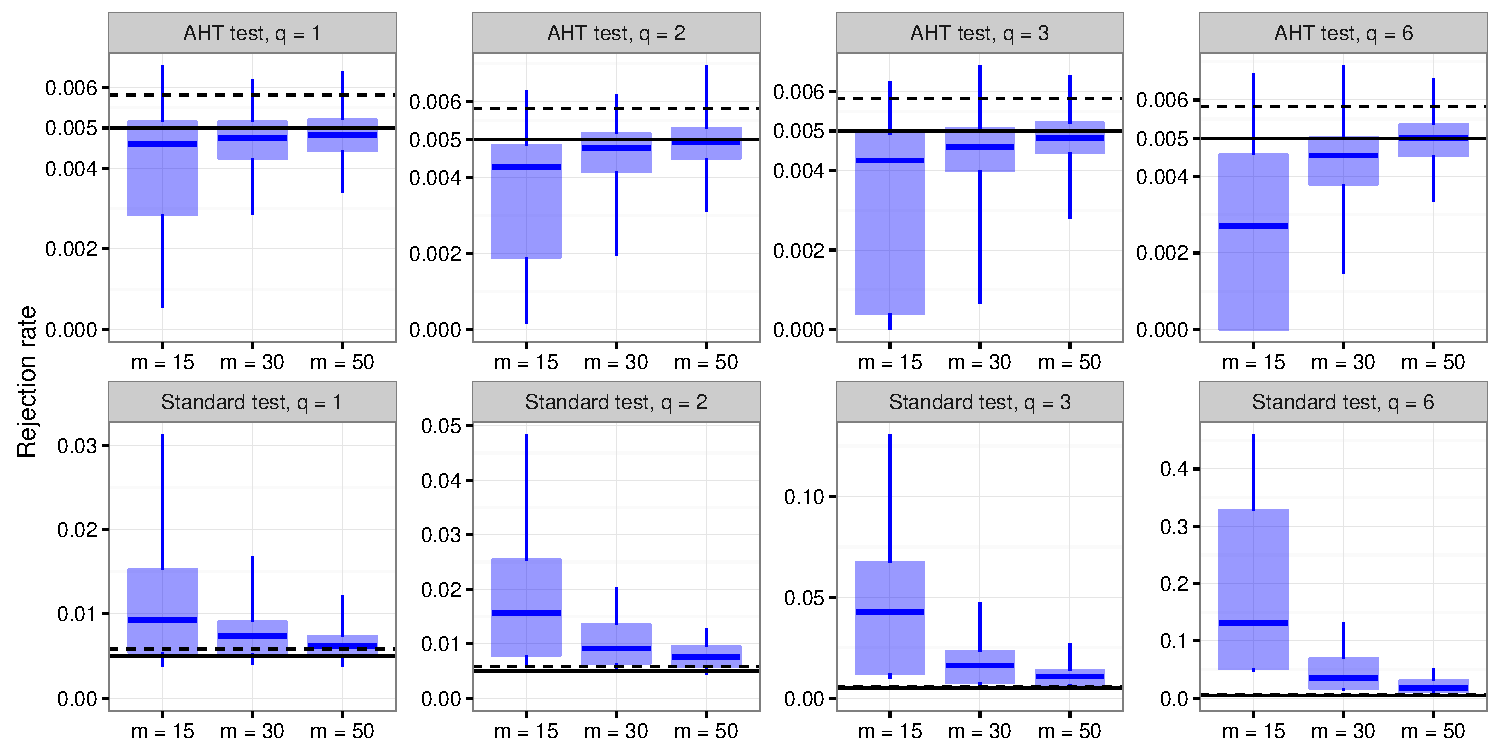
\includegraphics[width=\linewidth]{CR_fig/overview_005-1} 

}

\caption[Rejection rates of ad hoc and AHT tests for ]{Rejection rates of ad hoc and AHT tests for $\alpha = .005$, by dimension of hypothesis ($q$) and sample size ($m$).}\label{fig:overview_005}
\end{figure}


\end{knitrout}

\begin{knitrout}
\definecolor{shadecolor}{rgb}{0.969, 0.969, 0.969}\color{fgcolor}\begin{figure}[H]

{\centering 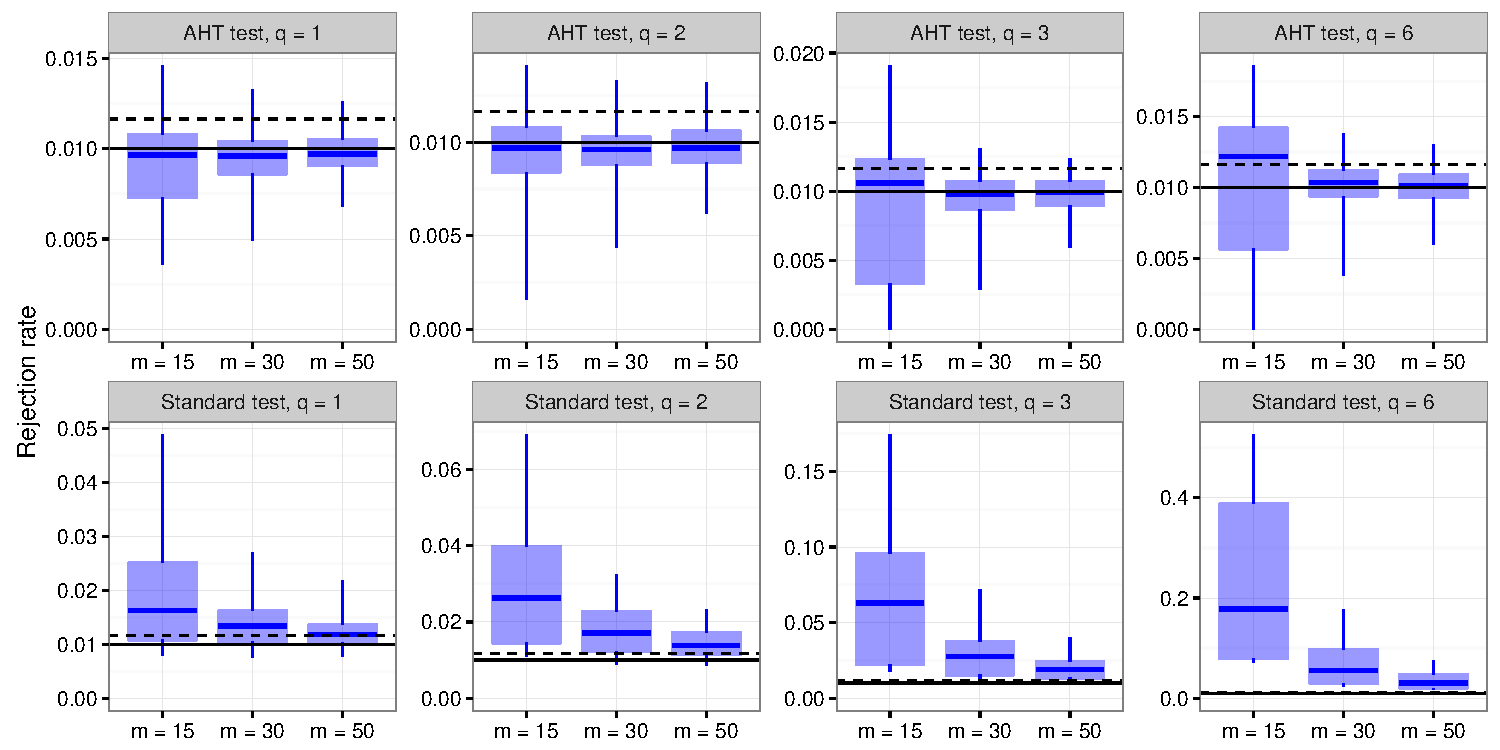
\includegraphics[width=\linewidth]{CR_fig/overview_01-1} 

}

\caption[Rejection rates of ad hoc and AHT tests for ]{Rejection rates of ad hoc and AHT tests for $\alpha = .01$, by dimension of hypothesis ($q$) and sample size ($m$).}\label{fig:overview_01}
\end{figure}


\end{knitrout}

\begin{knitrout}
\definecolor{shadecolor}{rgb}{0.969, 0.969, 0.969}\color{fgcolor}\begin{figure}[H]

{\centering 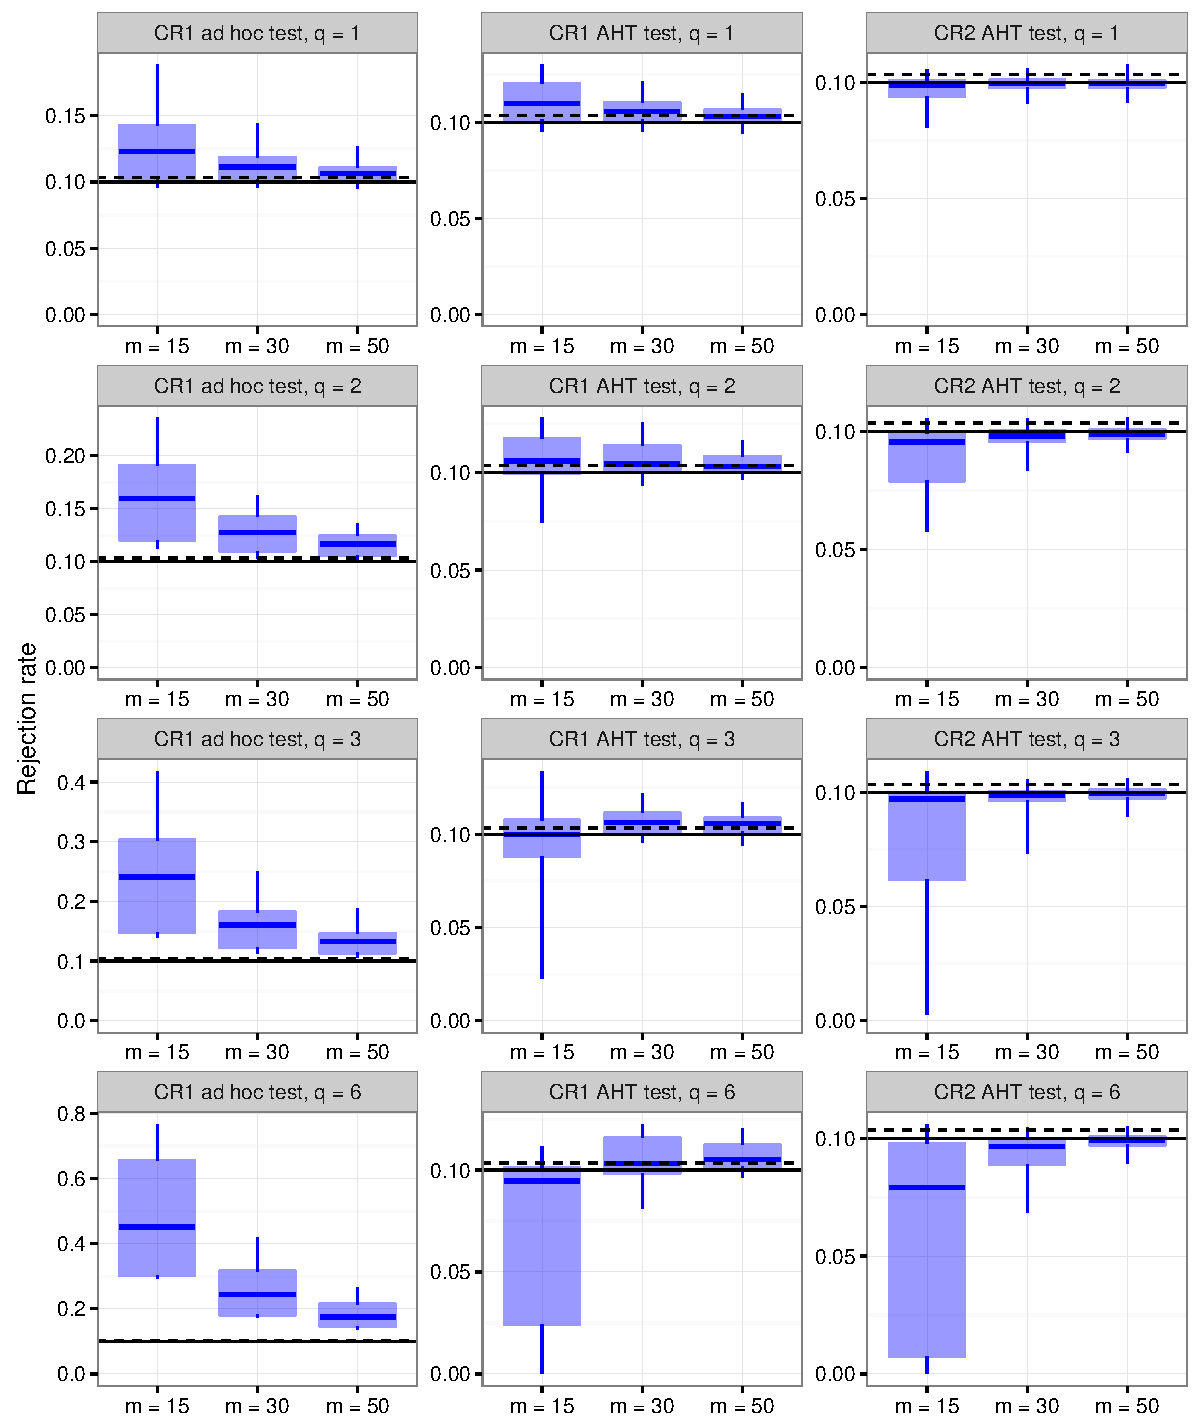
\includegraphics[width=\linewidth]{CR_fig/overview_10-1} 

}

\caption[Rejection rates of ad hoc and AHT tests for ]{Rejection rates of ad hoc and AHT tests for $\alpha = .10$, by dimension of hypothesis ($q$) and sample size ($m$).}\label{fig:overview_10}
\end{figure}


\end{knitrout}

\begin{knitrout}
\definecolor{shadecolor}{rgb}{0.969, 0.969, 0.969}\color{fgcolor}\begin{figure}[H]

{\centering 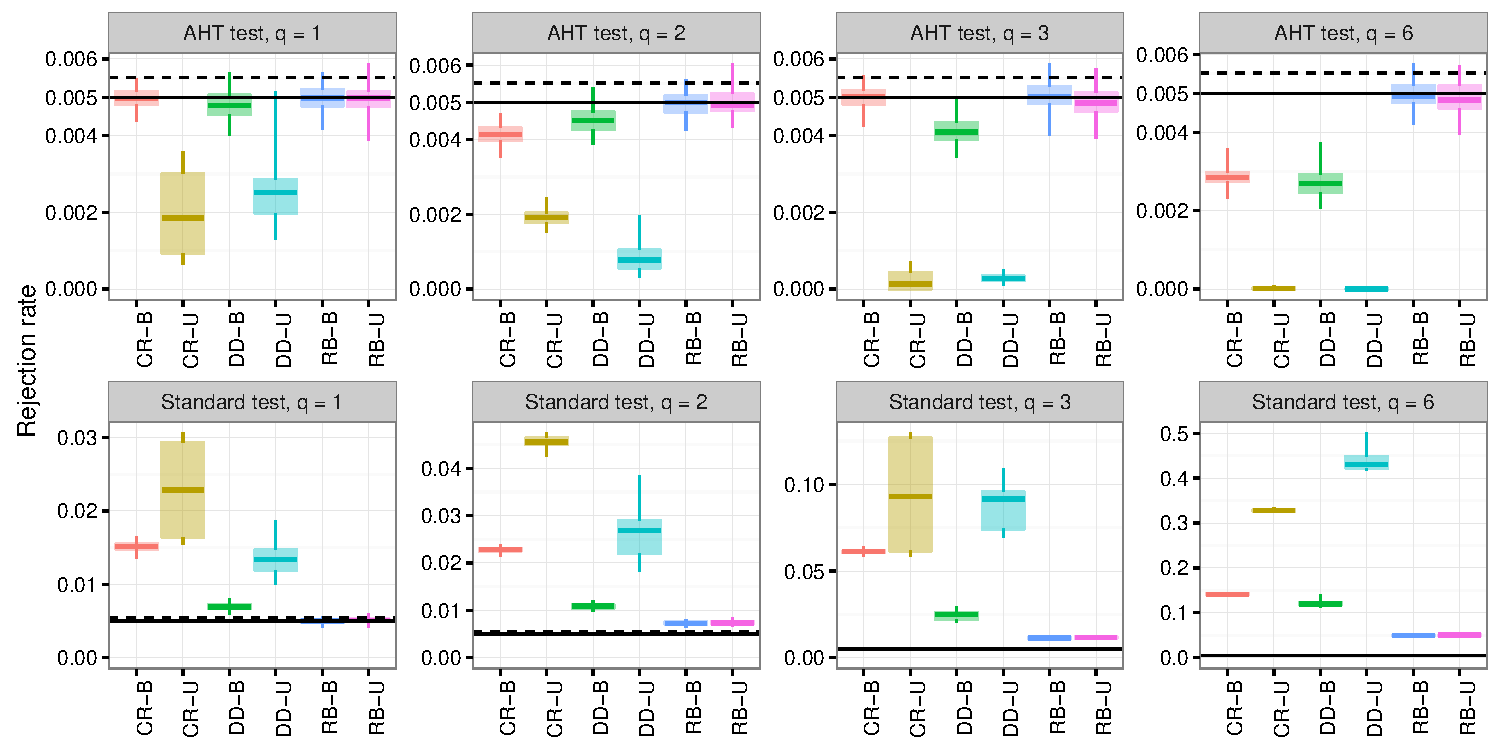
\includegraphics[width=\linewidth]{CR_fig/balance_005_15-1} 

}

\caption[Rejection rates of ad hoc and AHT tests, by study design and dimension of hypothesis (]{Rejection rates of ad hoc and AHT tests, by study design and dimension of hypothesis ($q$) for $\alpha = .005$ and $m = 15$. CR = cluster-randomized design; DD = difference-in-differences design; RB = randomized block design; B = balanced; U = unbalanced.}\label{fig:balance_005_15}
\end{figure}


\end{knitrout}

\begin{knitrout}
\definecolor{shadecolor}{rgb}{0.969, 0.969, 0.969}\color{fgcolor}\begin{figure}[H]

{\centering 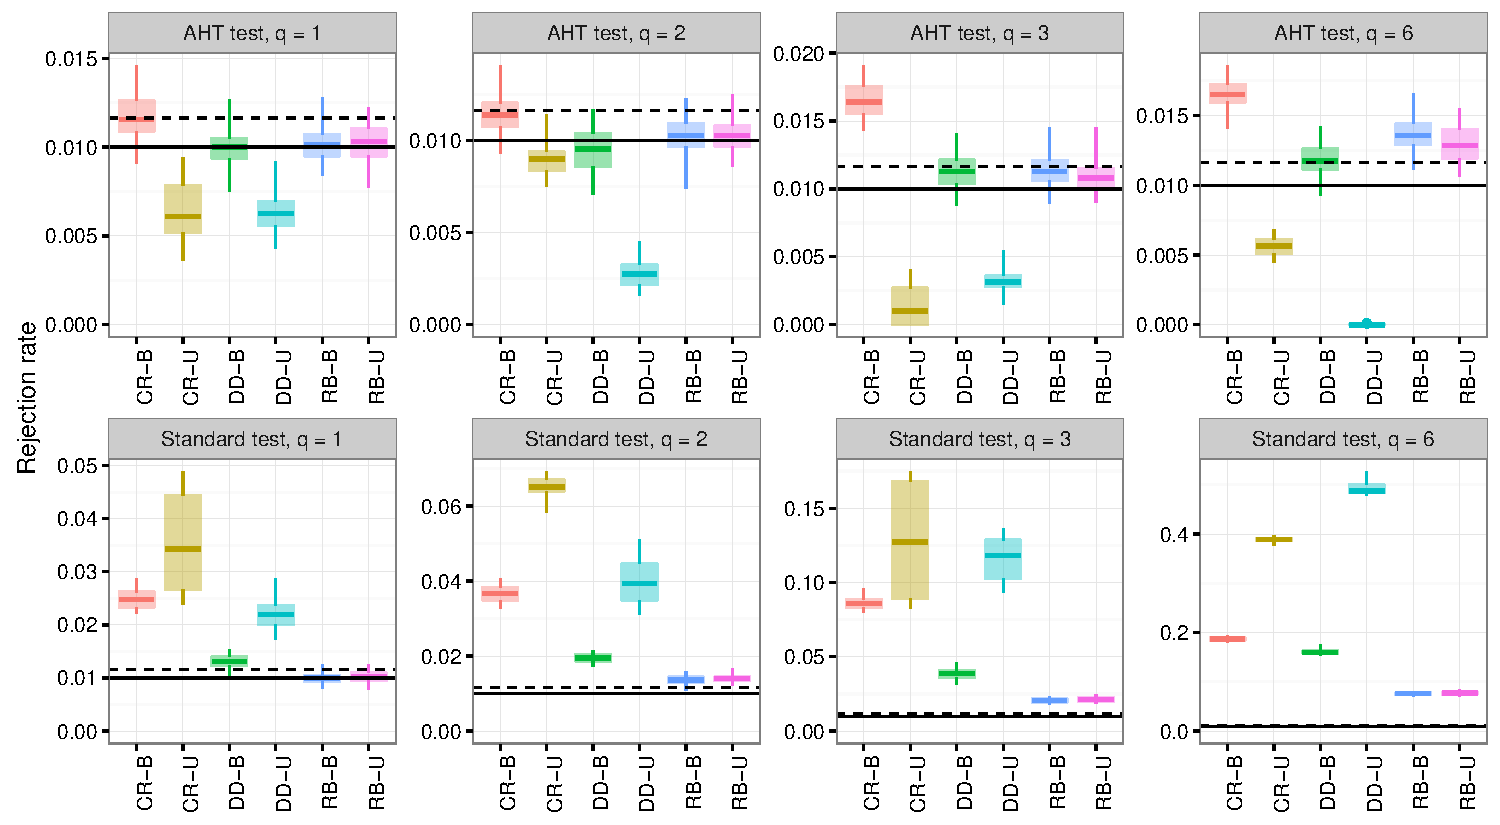
\includegraphics[width=\linewidth]{CR_fig/balance_01_15-1} 

}

\caption[Rejection rates of ad hoc and AHT tests, by study design and dimension of hypothesis (]{Rejection rates of ad hoc and AHT tests, by study design and dimension of hypothesis ($q$) for $\alpha = .01$ and $m = 15$. CR = cluster-randomized design; DD = difference-in-differences design; RB = randomized block design; B = balanced; U = unbalanced.}\label{fig:balance_01_15}
\end{figure}


\end{knitrout}

\begin{knitrout}
\definecolor{shadecolor}{rgb}{0.969, 0.969, 0.969}\color{fgcolor}\begin{figure}[H]

{\centering 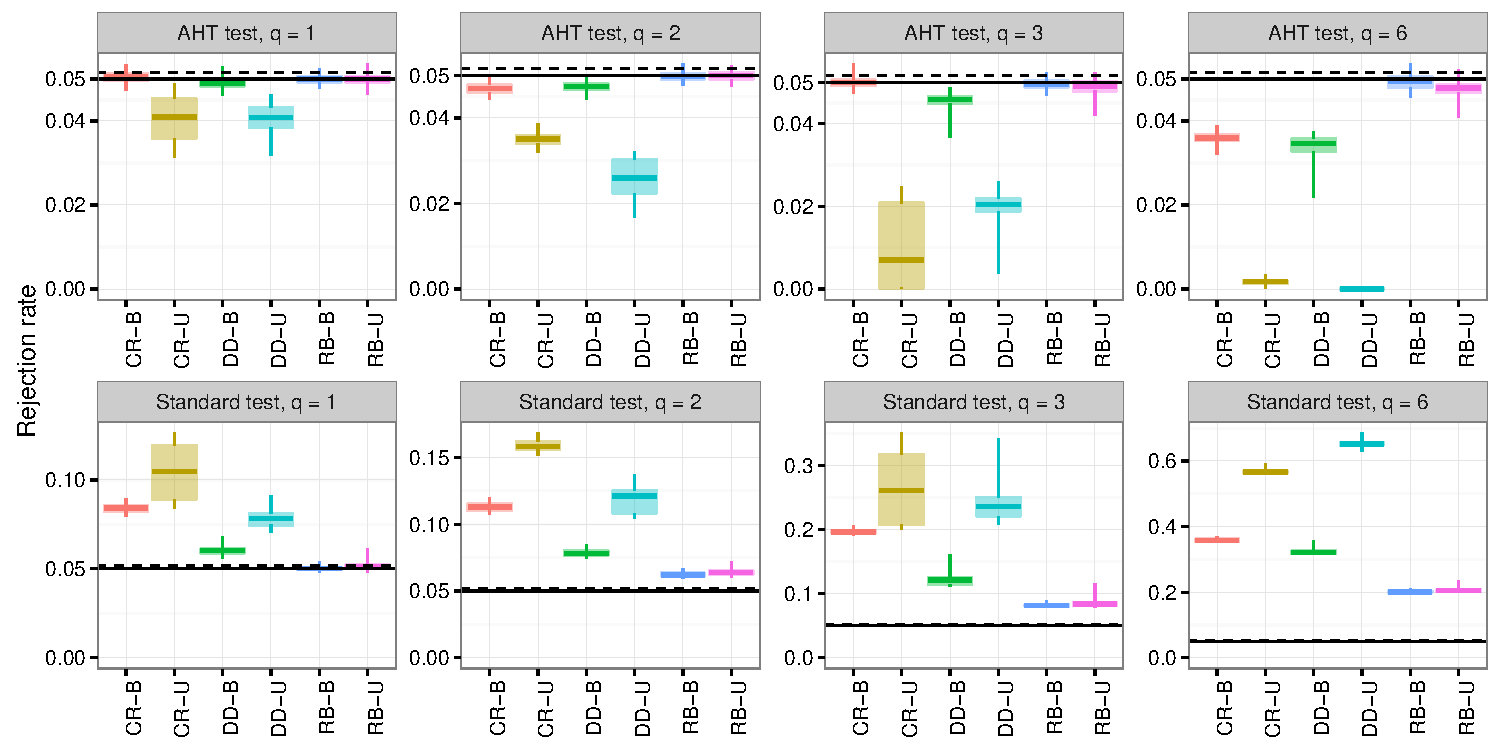
\includegraphics[width=\linewidth]{CR_fig/balance_05_15-1} 

}

\caption[Rejection rates of ad hoc and AHT tests, by study design and dimension of hypothesis (]{Rejection rates of ad hoc and AHT tests, by study design and dimension of hypothesis ($q$) for $\alpha = .05$ and $m = 15$. CR = cluster-randomized design; DD = difference-in-differences design; RB = randomized block design; B = balanced; U = unbalanced.}\label{fig:balance_05_15}
\end{figure}


\end{knitrout}

\begin{knitrout}
\definecolor{shadecolor}{rgb}{0.969, 0.969, 0.969}\color{fgcolor}\begin{figure}[H]

{\centering 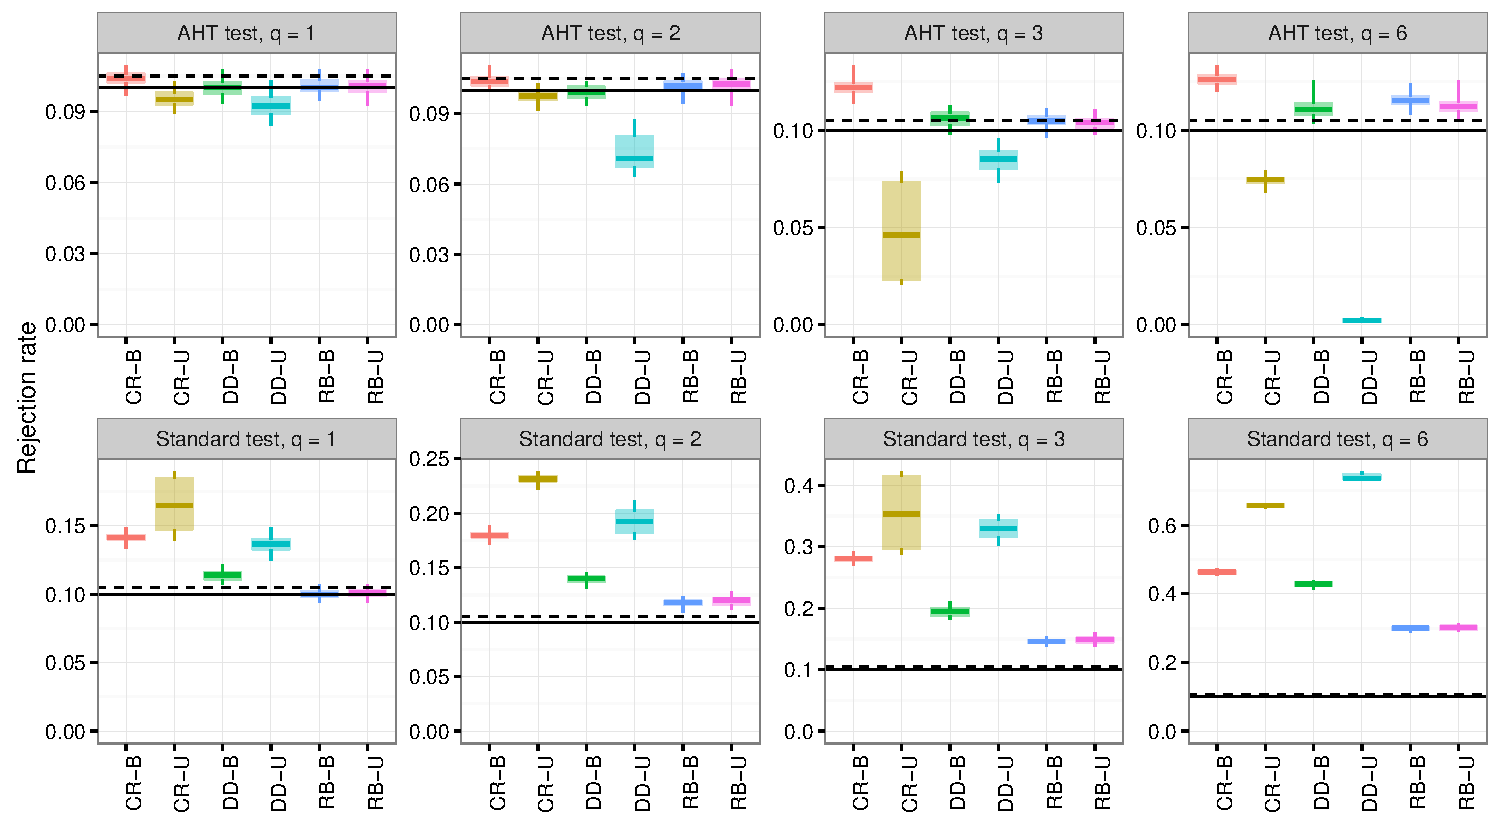
\includegraphics[width=\linewidth]{CR_fig/balance_10_15-1} 

}

\caption[Rejection rates of ad hoc and AHT tests, by study design and dimension of hypothesis (]{Rejection rates of ad hoc and AHT tests, by study design and dimension of hypothesis ($q$) for $\alpha = .10$ and $m = 15$. CR = cluster-randomized design; DD = difference-in-differences design; RB = randomized block design; B = balanced; U = unbalanced.}\label{fig:balance_10_15}
\end{figure}


\end{knitrout}

\begin{knitrout}
\definecolor{shadecolor}{rgb}{0.969, 0.969, 0.969}\color{fgcolor}\begin{figure}[H]

{\centering 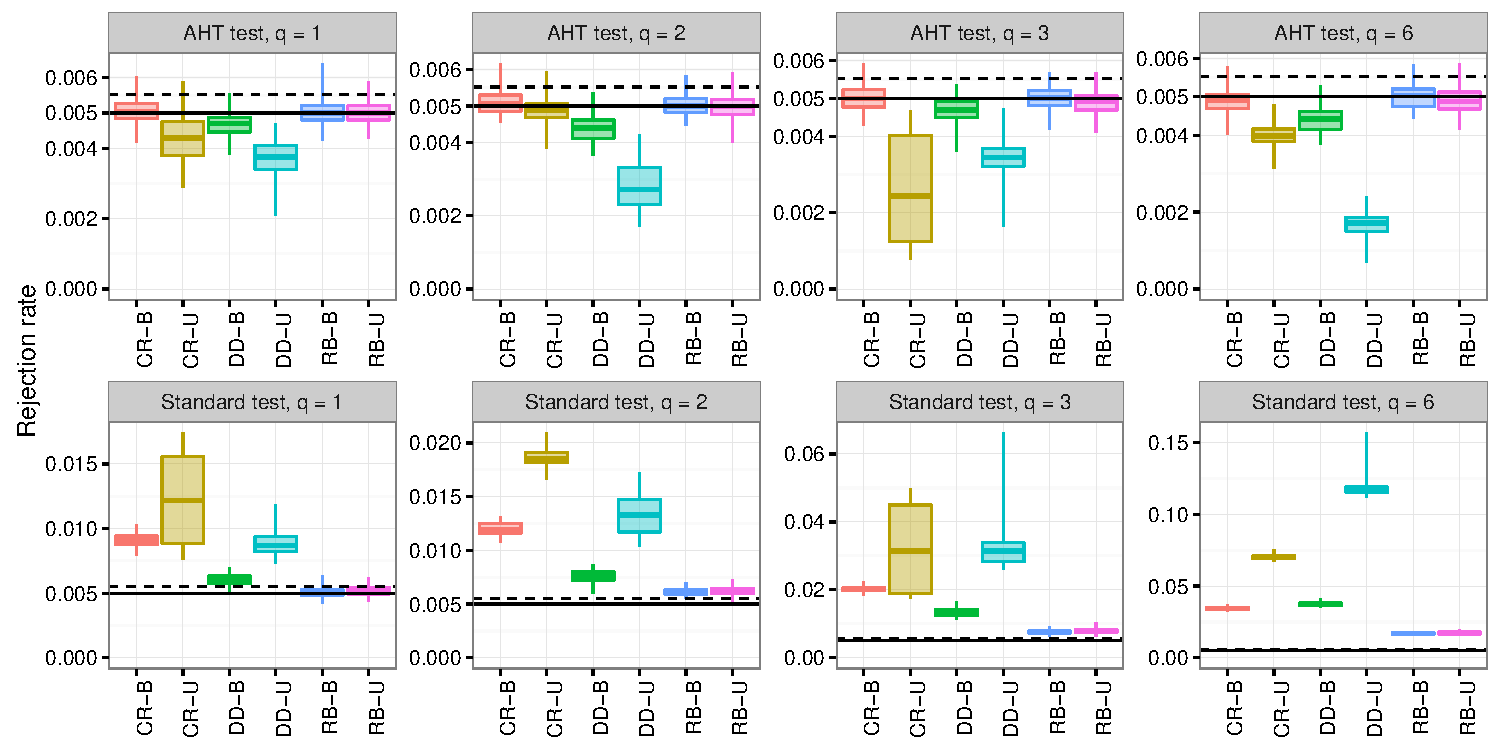
\includegraphics[width=\linewidth]{CR_fig/balance_005_30-1} 

}

\caption[Rejection rates of ad hoc and AHT tests, by study design and dimension of hypothesis (]{Rejection rates of ad hoc and AHT tests, by study design and dimension of hypothesis ($q$) for $\alpha = .005$ and $m = 30$. CR = cluster-randomized design; DD = difference-in-differences design; RB = randomized block design; B = balanced; U = unbalanced.}\label{fig:balance_005_30}
\end{figure}


\end{knitrout}

\begin{knitrout}
\definecolor{shadecolor}{rgb}{0.969, 0.969, 0.969}\color{fgcolor}\begin{figure}[H]

{\centering 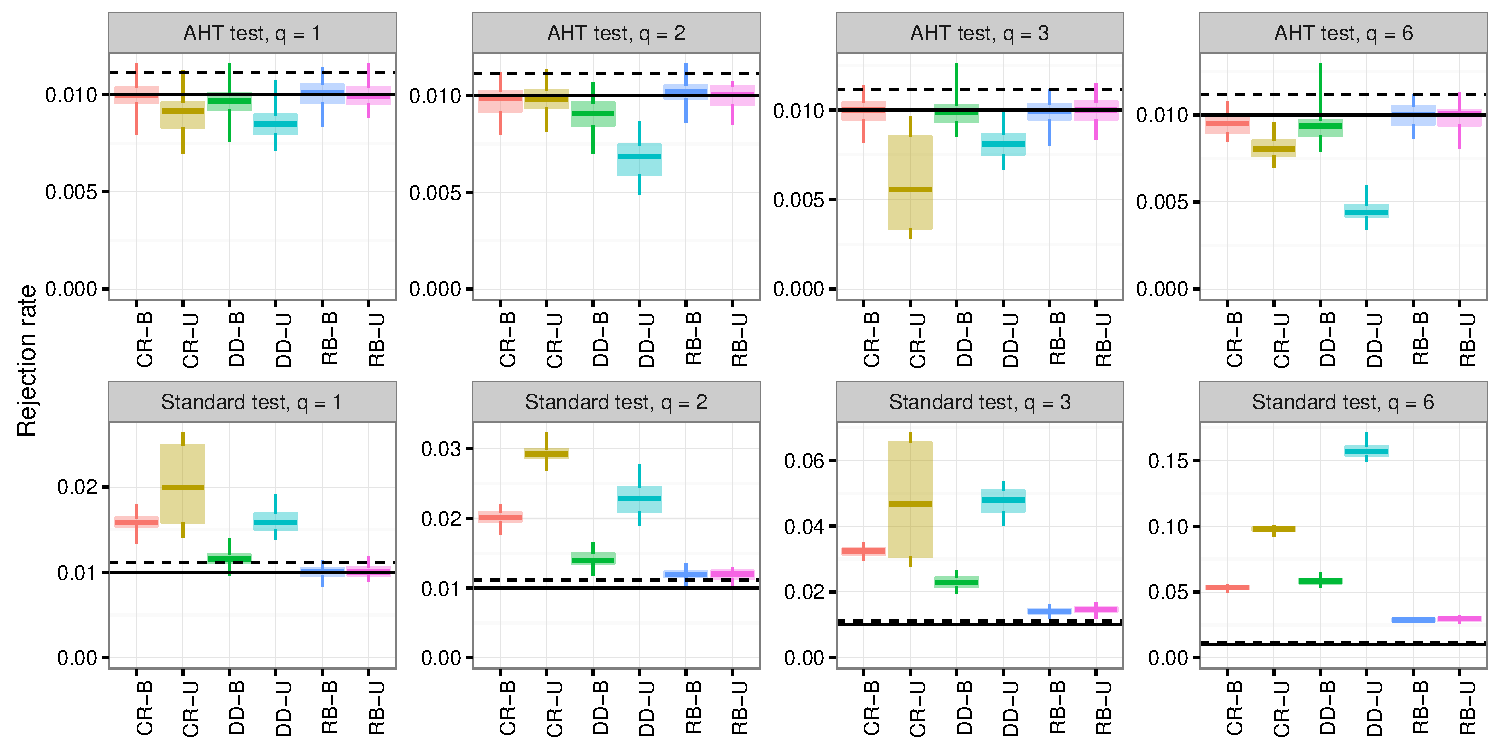
\includegraphics[width=\linewidth]{CR_fig/balance_01_30-1} 

}

\caption[Rejection rates of ad hoc and AHT tests, by study design and dimension of hypothesis (]{Rejection rates of ad hoc and AHT tests, by study design and dimension of hypothesis ($q$) for $\alpha = .01$ and $m = 30$. CR = cluster-randomized design; DD = difference-in-differences design; RB = randomized block design; B = balanced; U = unbalanced.}\label{fig:balance_01_30}
\end{figure}


\end{knitrout}

\begin{knitrout}
\definecolor{shadecolor}{rgb}{0.969, 0.969, 0.969}\color{fgcolor}\begin{figure}[H]

{\centering 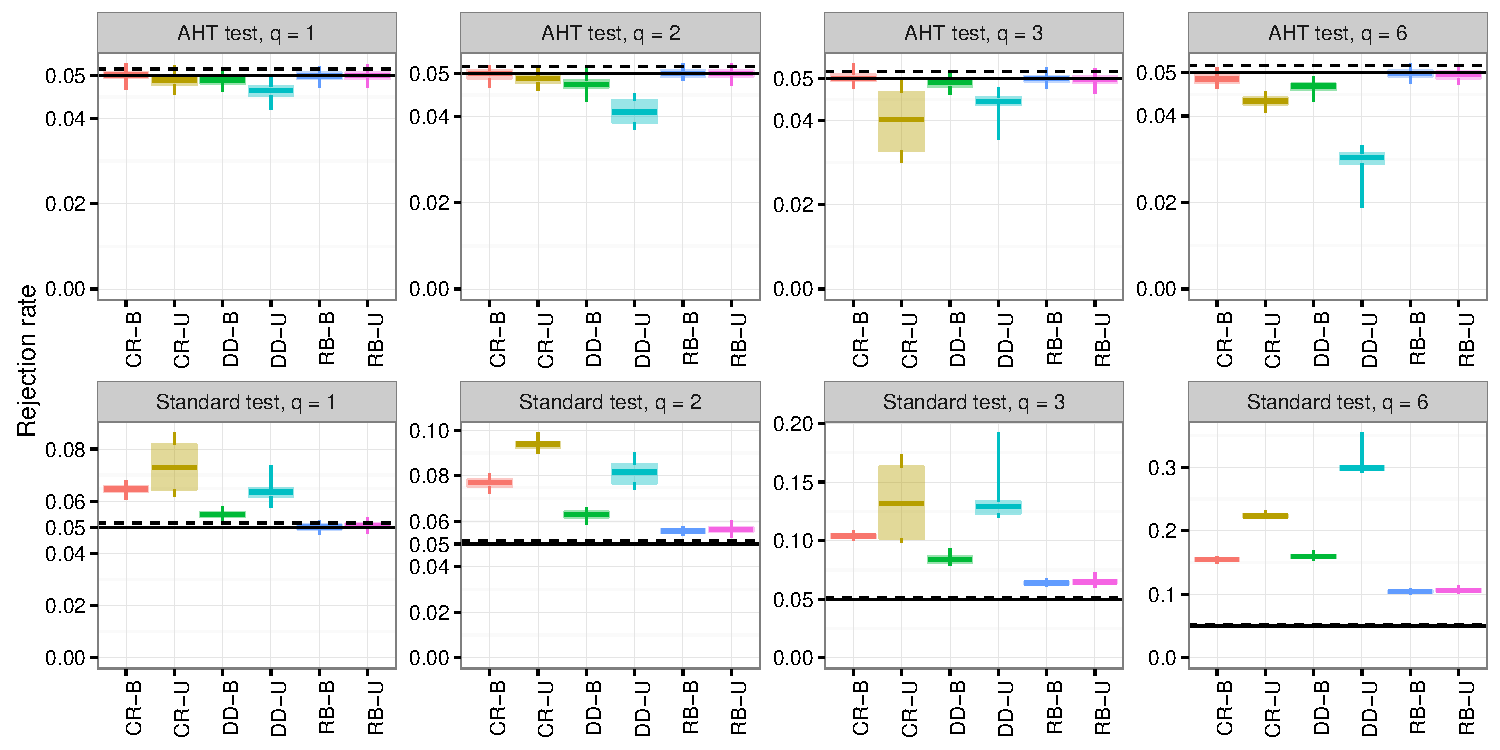
\includegraphics[width=\linewidth]{CR_fig/balance_05_30-1} 

}

\caption[Rejection rates of ad hoc and AHT tests, by study design and dimension of hypothesis (]{Rejection rates of ad hoc and AHT tests, by study design and dimension of hypothesis ($q$) for $\alpha = .05$ and $m = 30$. CR = cluster-randomized design; DD = difference-in-differences design; RB = randomized block design; B = balanced; U = unbalanced.}\label{fig:balance_05_30}
\end{figure}


\end{knitrout}

\begin{knitrout}
\definecolor{shadecolor}{rgb}{0.969, 0.969, 0.969}\color{fgcolor}\begin{figure}[H]

{\centering 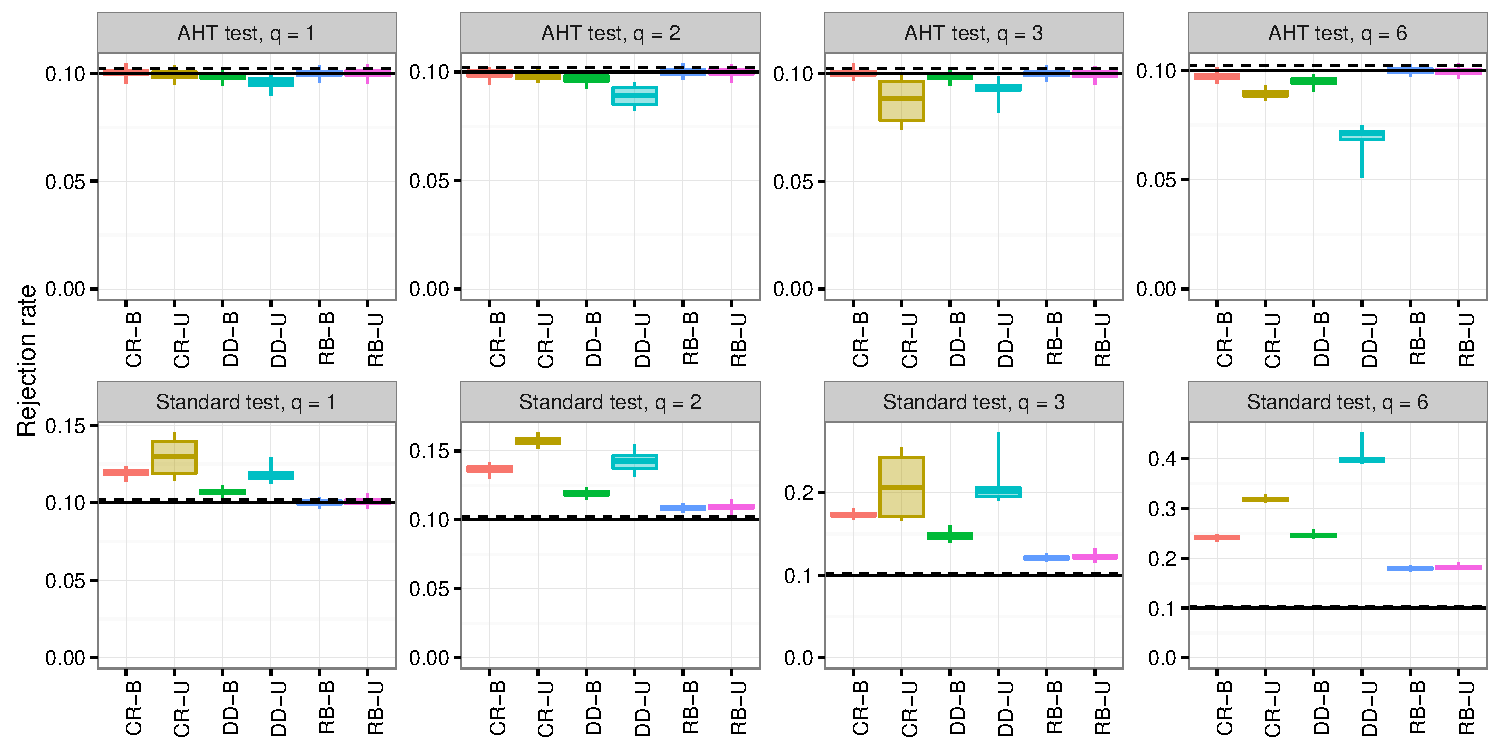
\includegraphics[width=\linewidth]{CR_fig/balance_10_30-1} 

}

\caption[Rejection rates of ad hoc and AHT tests, by study design and dimension of hypothesis (]{Rejection rates of ad hoc and AHT tests, by study design and dimension of hypothesis ($q$) for $\alpha = .10$ and $m = 30$. CR = cluster-randomized design; DD = difference-in-differences design; RB = randomized block design; B = balanced; U = unbalanced.}\label{fig:balance_10_30}
\end{figure}


\end{knitrout}

\begin{knitrout}
\definecolor{shadecolor}{rgb}{0.969, 0.969, 0.969}\color{fgcolor}\begin{figure}[H]

{\centering 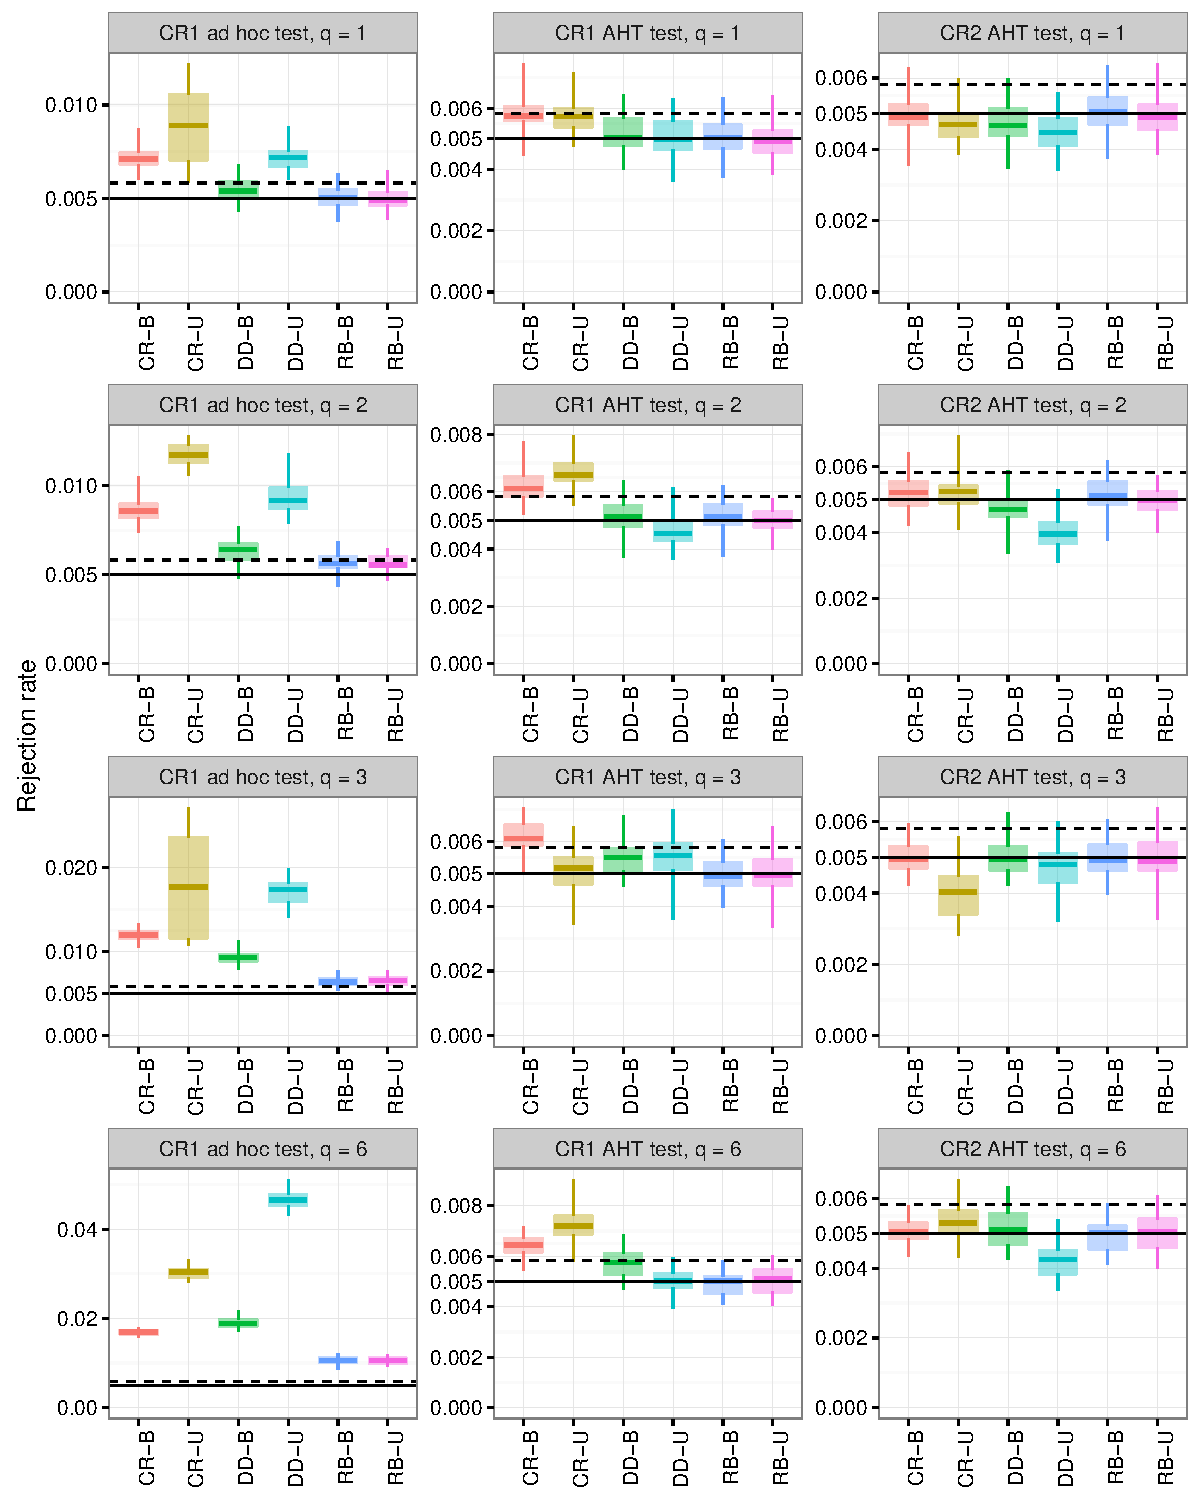
\includegraphics[width=\linewidth]{CR_fig/balance_005_50-1} 

}

\caption[Rejection rates of ad hoc and AHT tests, by study design and dimension of hypothesis (]{Rejection rates of ad hoc and AHT tests, by study design and dimension of hypothesis ($q$) for $\alpha = .005$ and $m = 50$. CR = cluster-randomized design; DD = difference-in-differences design; RB = randomized block design; B = balanced; U = unbalanced.}\label{fig:balance_005_50}
\end{figure}


\end{knitrout}

\begin{knitrout}
\definecolor{shadecolor}{rgb}{0.969, 0.969, 0.969}\color{fgcolor}\begin{figure}[H]

{\centering 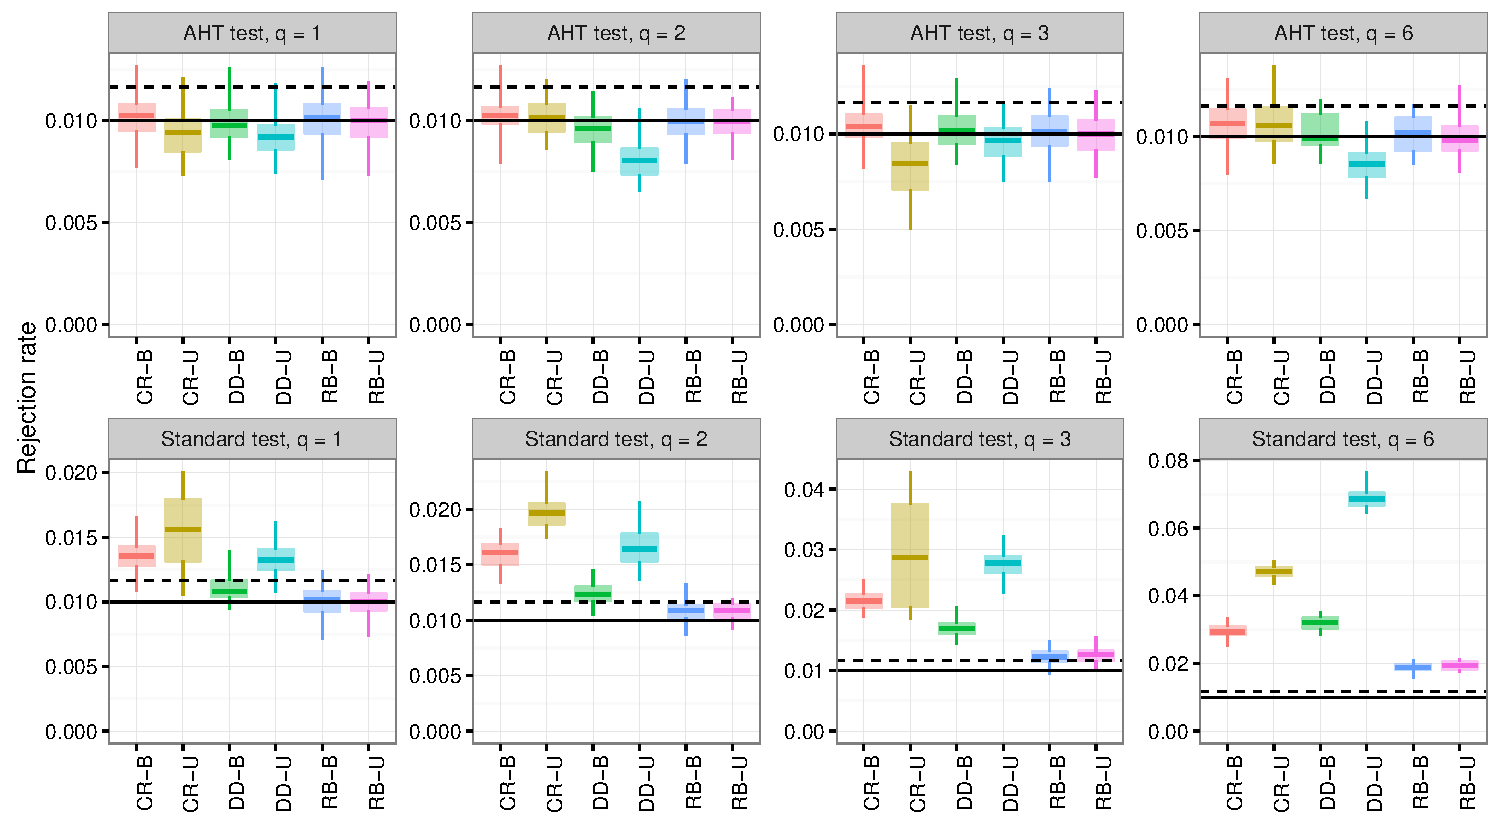
\includegraphics[width=\linewidth]{CR_fig/balance_01_50-1} 

}

\caption[Rejection rates of ad hoc and AHT tests, by study design and dimension of hypothesis (]{Rejection rates of ad hoc and AHT tests, by study design and dimension of hypothesis ($q$) for $\alpha = .01$ and $m = 50$. CR = cluster-randomized design; DD = difference-in-differences design; RB = randomized block design; B = balanced; U = unbalanced.}\label{fig:balance_01_50}
\end{figure}


\end{knitrout}

\begin{knitrout}
\definecolor{shadecolor}{rgb}{0.969, 0.969, 0.969}\color{fgcolor}\begin{figure}[H]

{\centering 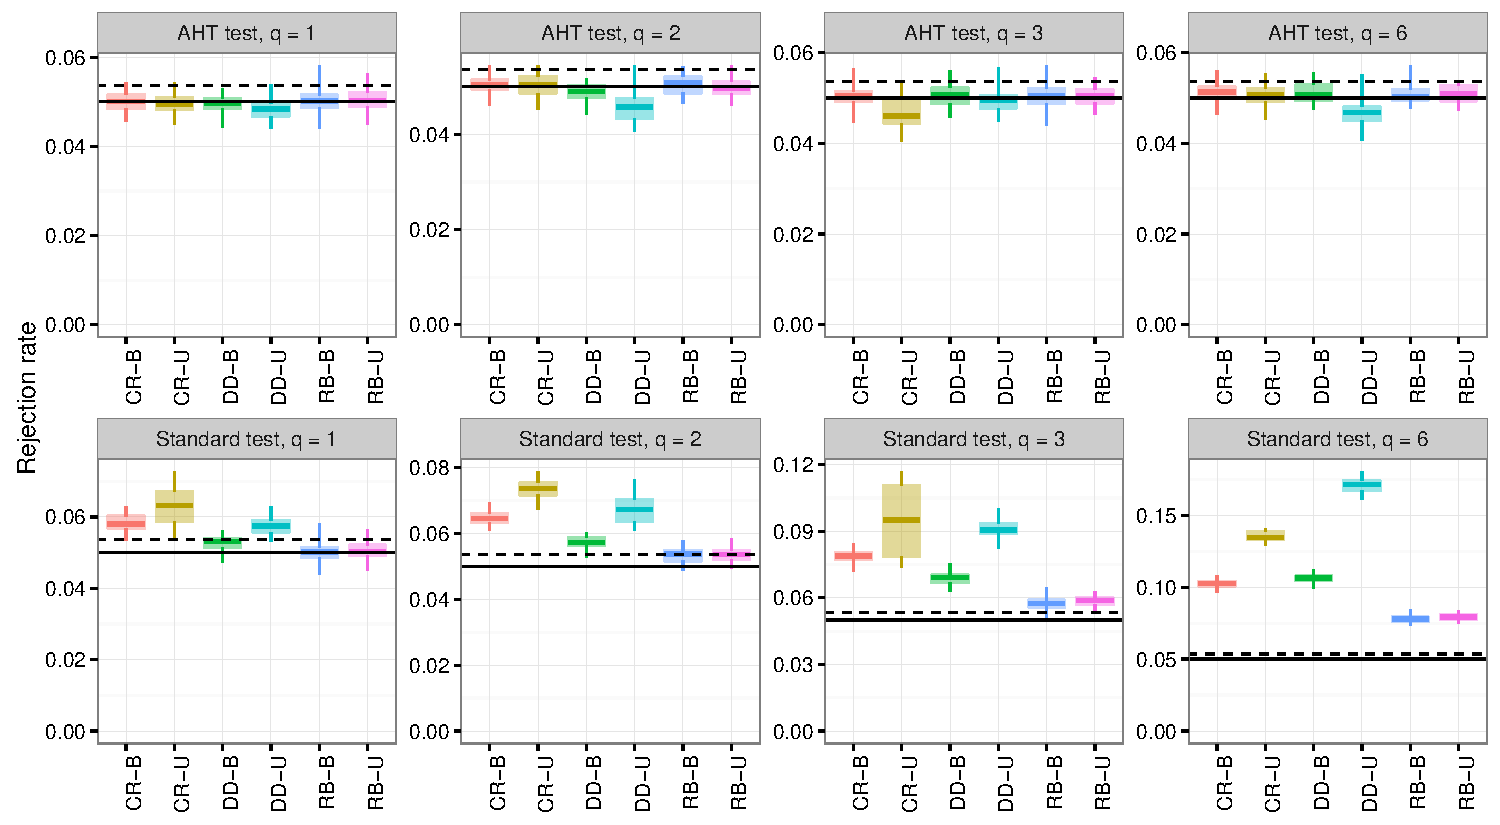
\includegraphics[width=\linewidth]{CR_fig/balance_05_50-1} 

}

\caption[Rejection rates of ad hoc and AHT tests, by study design and dimension of hypothesis (]{Rejection rates of ad hoc and AHT tests, by study design and dimension of hypothesis ($q$) for $\alpha = .05$ and $m = 50$. CR = cluster-randomized design; DD = difference-in-differences design; RB = randomized block design; B = balanced; U = unbalanced.}\label{fig:balance_05_50}
\end{figure}


\end{knitrout}

\begin{knitrout}
\definecolor{shadecolor}{rgb}{0.969, 0.969, 0.969}\color{fgcolor}\begin{figure}[H]

{\centering 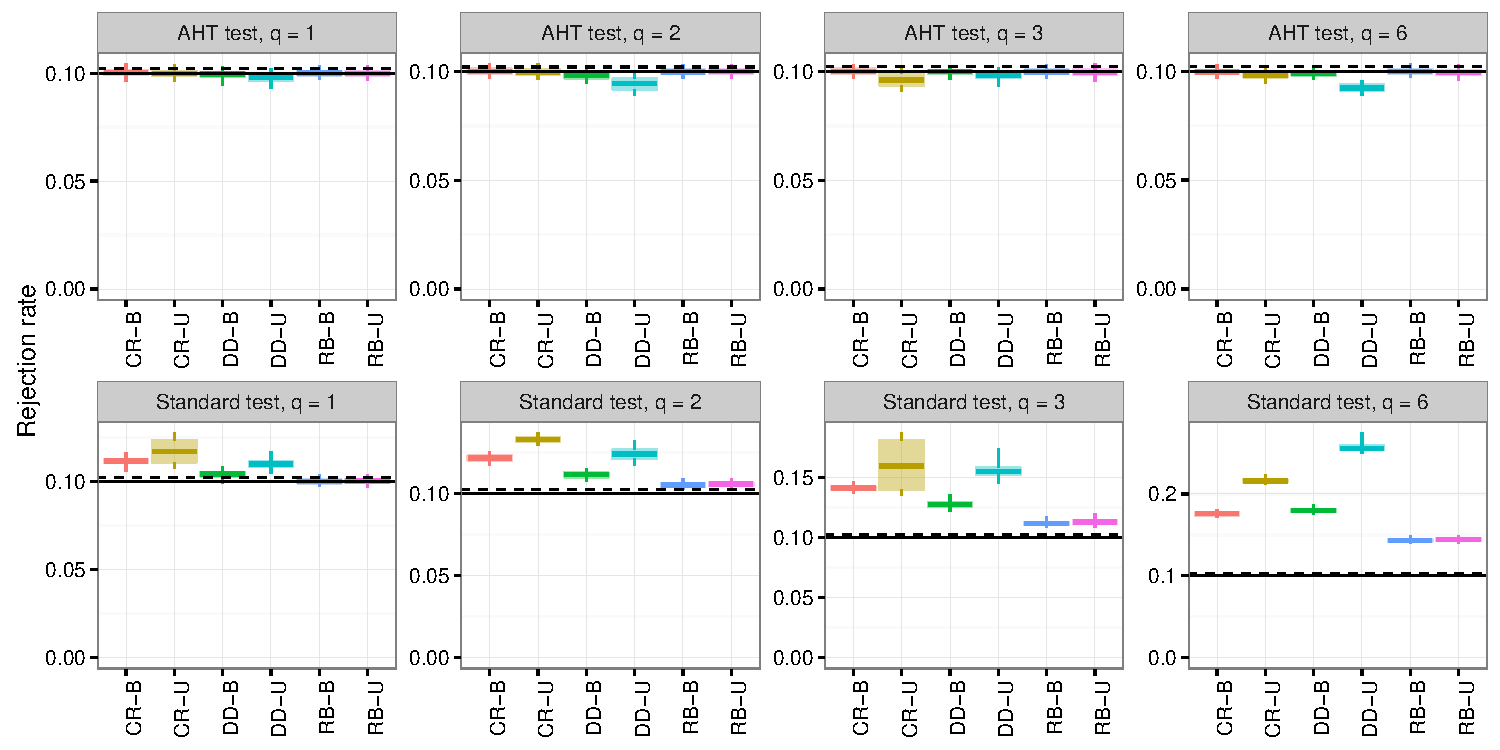
\includegraphics[width=\linewidth]{CR_fig/balance_10_50-1} 

}

\caption[Rejection rates of ad hoc and AHT tests, by study design and dimension of hypothesis (]{Rejection rates of ad hoc and AHT tests, by study design and dimension of hypothesis ($q$) for $\alpha = .10$ and $m = 50$. CR = cluster-randomized design; DD = difference-in-differences design; RB = randomized block design; B = balanced; U = unbalanced.}\label{fig:balance_10_50}
\end{figure}


\end{knitrout}

\begin{landscape}

\begin{knitrout}
\definecolor{shadecolor}{rgb}{0.969, 0.969, 0.969}\color{fgcolor}\begin{figure}[H]

{\centering 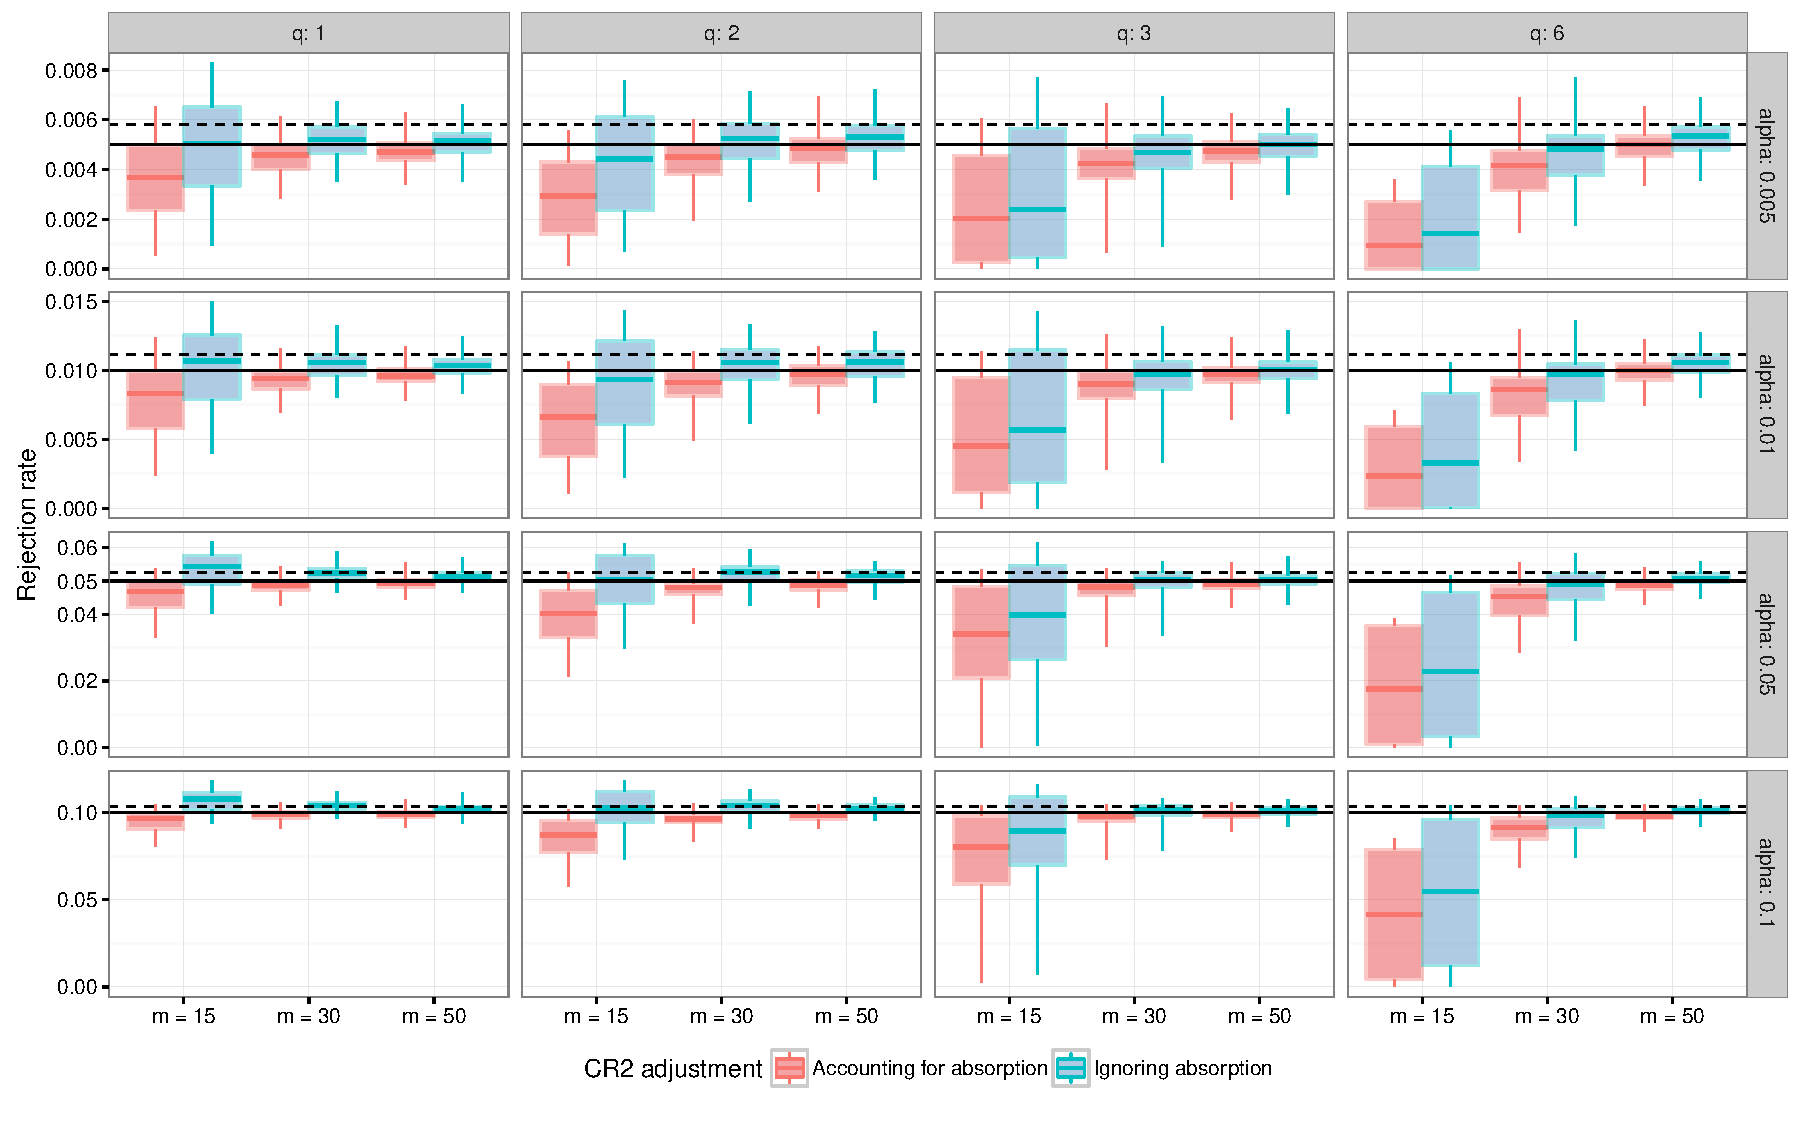
\includegraphics[width=\linewidth]{CR_fig/absorption-1} 

}

\caption[Rejection rates of AHT test using CR2, calculated with and without accounting for absorption of fixed effects, by sample size (]{Rejection rates of AHT test using CR2, calculated with and without accounting for absorption of fixed effects, by sample size ($m$), dimension of hypothesis ($q$), and $\alpha $-level. Results for the balanced and unbalanced randomized block designs are excluded because accounting for absorption of fixed effects has no consequence for these designs.}\label{fig:absorption}
\end{figure}


\end{knitrout}

\begin{knitrout}
\definecolor{shadecolor}{rgb}{0.969, 0.969, 0.969}\color{fgcolor}\begin{figure}[H]

{\centering 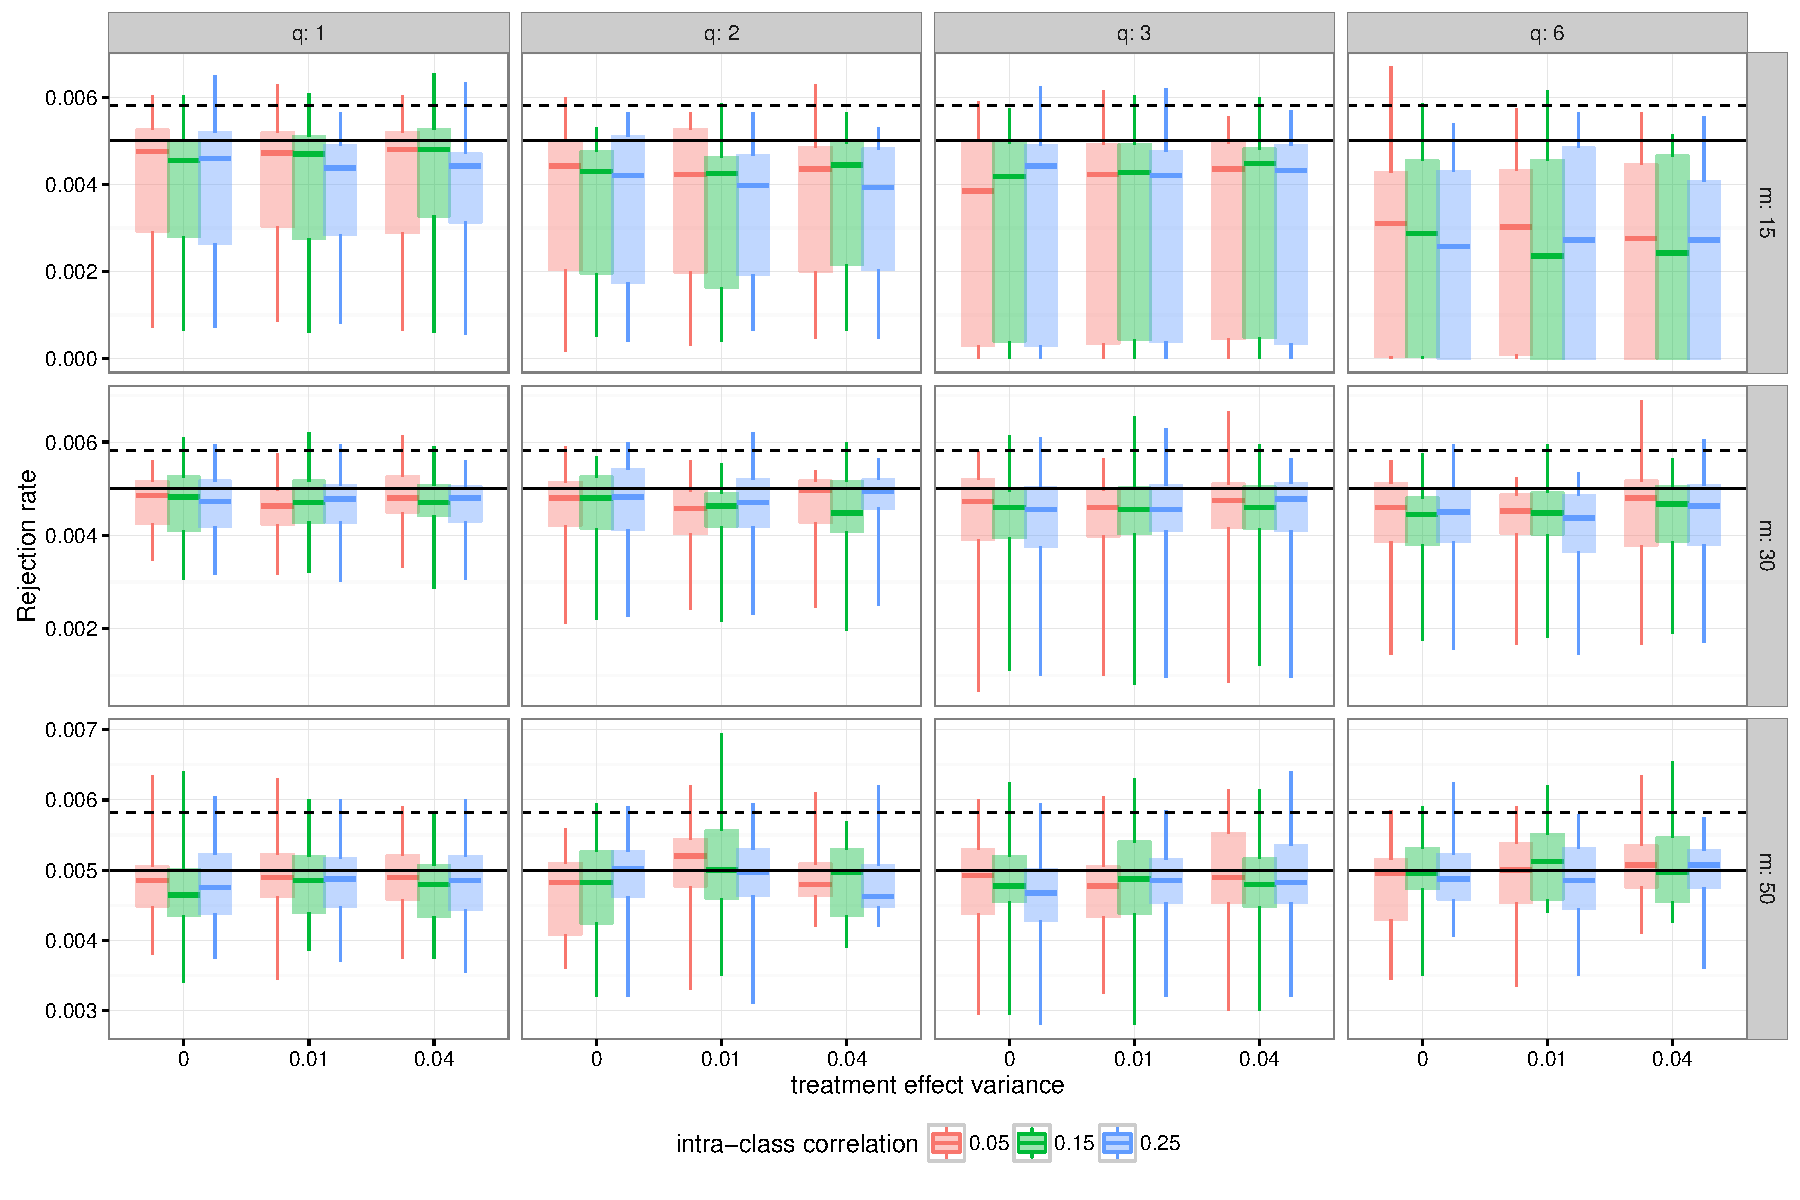
\includegraphics[width=\linewidth]{CR_fig/misspecification_005-1} 

}

\caption[Rejection rates of CR2 AHT test, by treatment effect variance and intra-class correlation for ]{Rejection rates of CR2 AHT test, by treatment effect variance and intra-class correlation for $\alpha = .005$.}\label{fig:misspecification_005}
\end{figure}


\end{knitrout}

\begin{knitrout}
\definecolor{shadecolor}{rgb}{0.969, 0.969, 0.969}\color{fgcolor}\begin{figure}[H]

{\centering 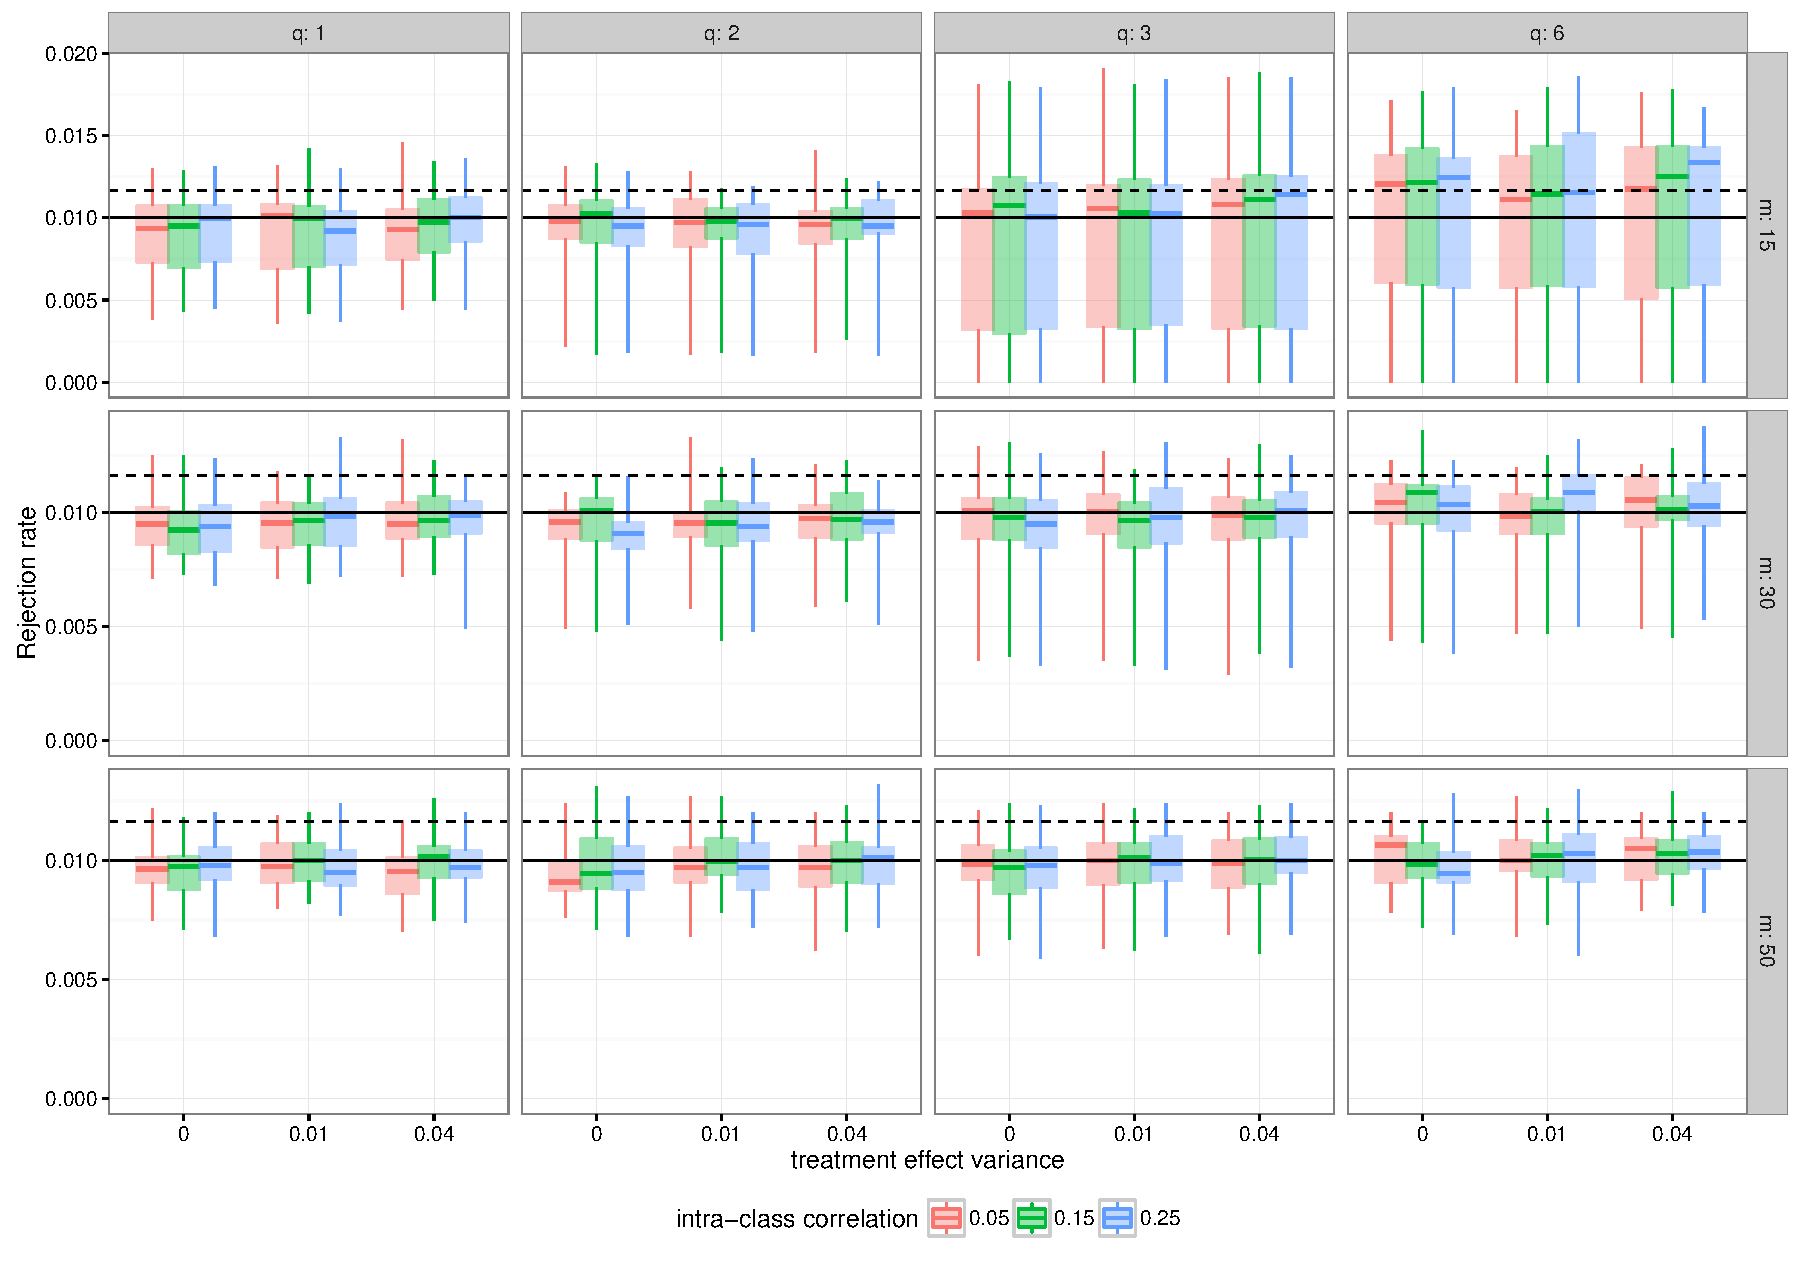
\includegraphics[width=\linewidth]{CR_fig/misspecification_01-1} 

}

\caption[Rejection rates of CR2 AHT test, by treatment effect variance and intra-class correlation for ]{Rejection rates of CR2 AHT test, by treatment effect variance and intra-class correlation for $\alpha = .01$.}\label{fig:misspecification_01}
\end{figure}


\end{knitrout}

\begin{knitrout}
\definecolor{shadecolor}{rgb}{0.969, 0.969, 0.969}\color{fgcolor}\begin{figure}[H]

{\centering 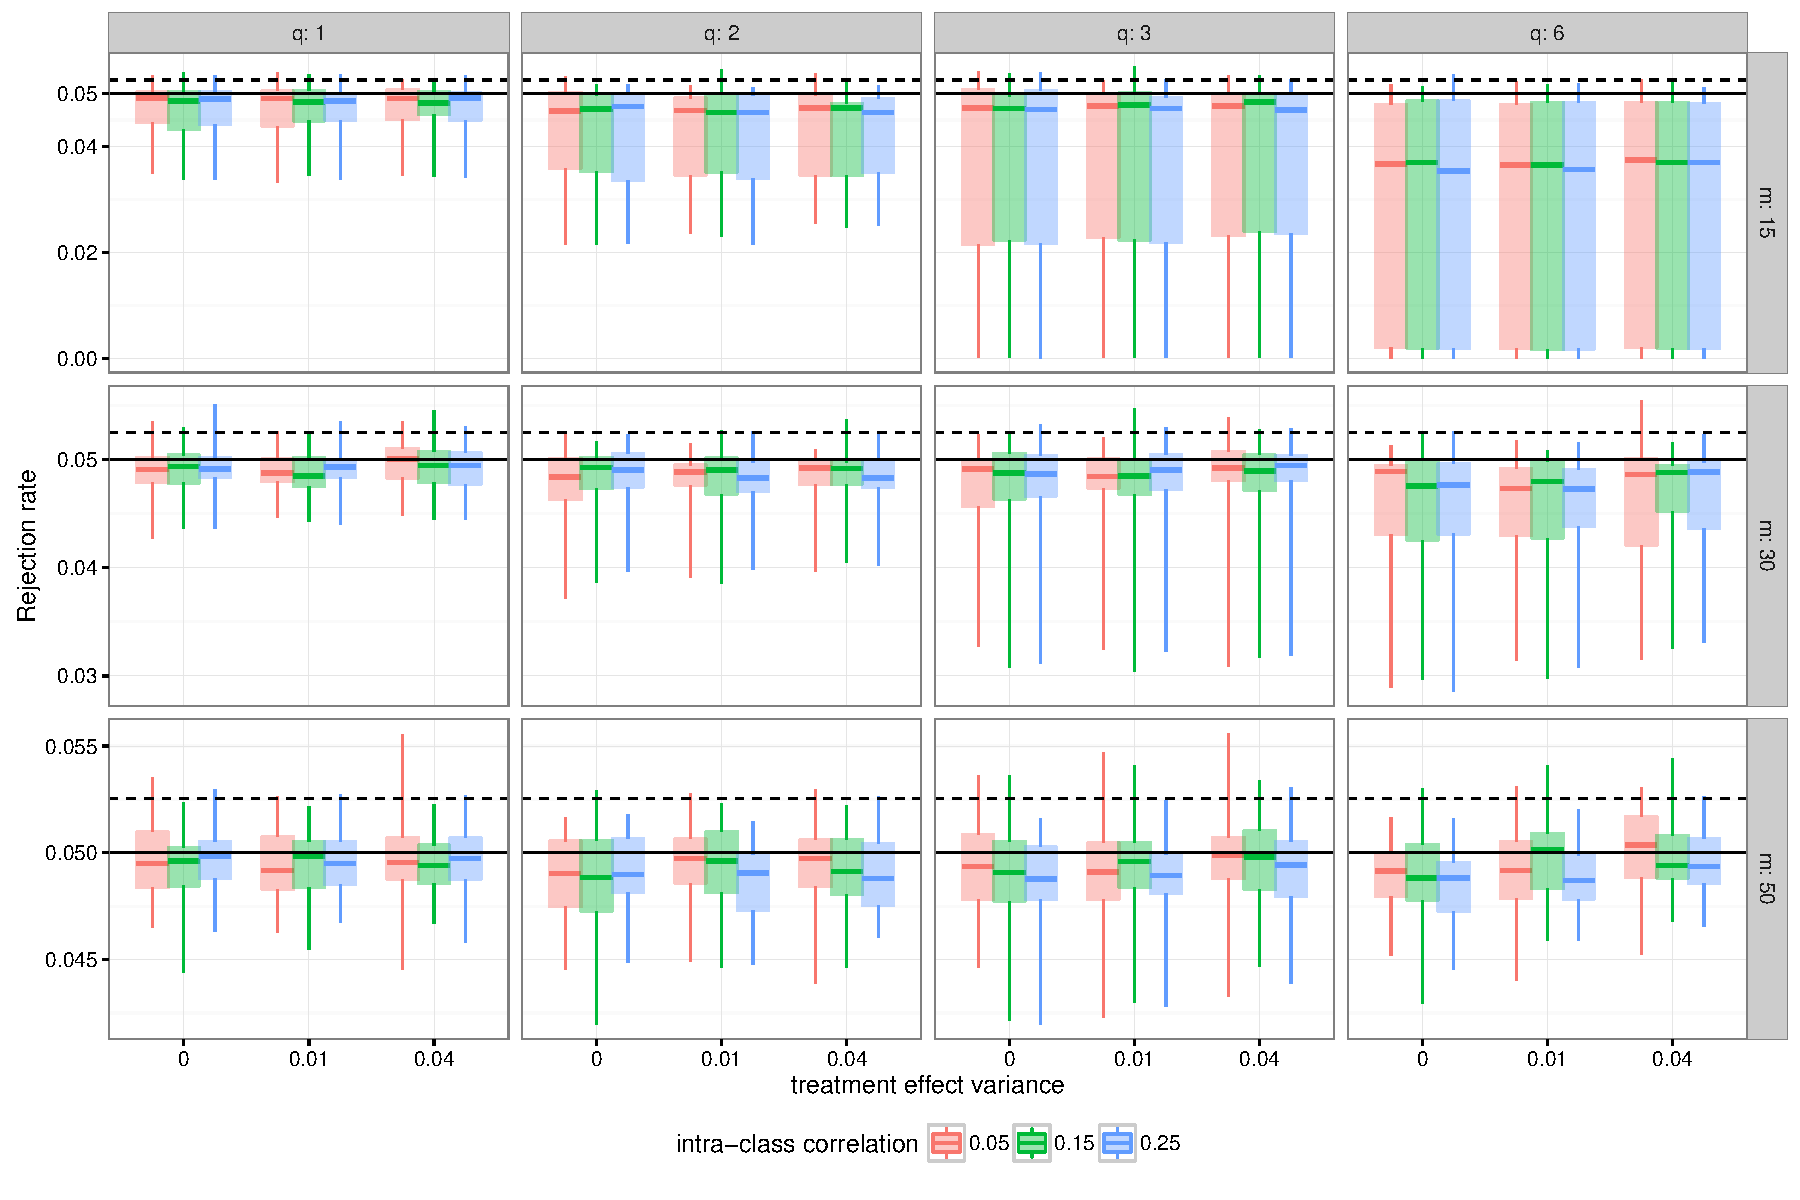
\includegraphics[width=\linewidth]{CR_fig/misspecification_05-1} 

}

\caption[Rejection rates of CR2 AHT test, by treatment effect variance and intra-class correlation for ]{Rejection rates of CR2 AHT test, by treatment effect variance and intra-class correlation for $\alpha = .05$.}\label{fig:misspecification_05}
\end{figure}


\end{knitrout}

\begin{knitrout}
\definecolor{shadecolor}{rgb}{0.969, 0.969, 0.969}\color{fgcolor}\begin{figure}[H]

{\centering 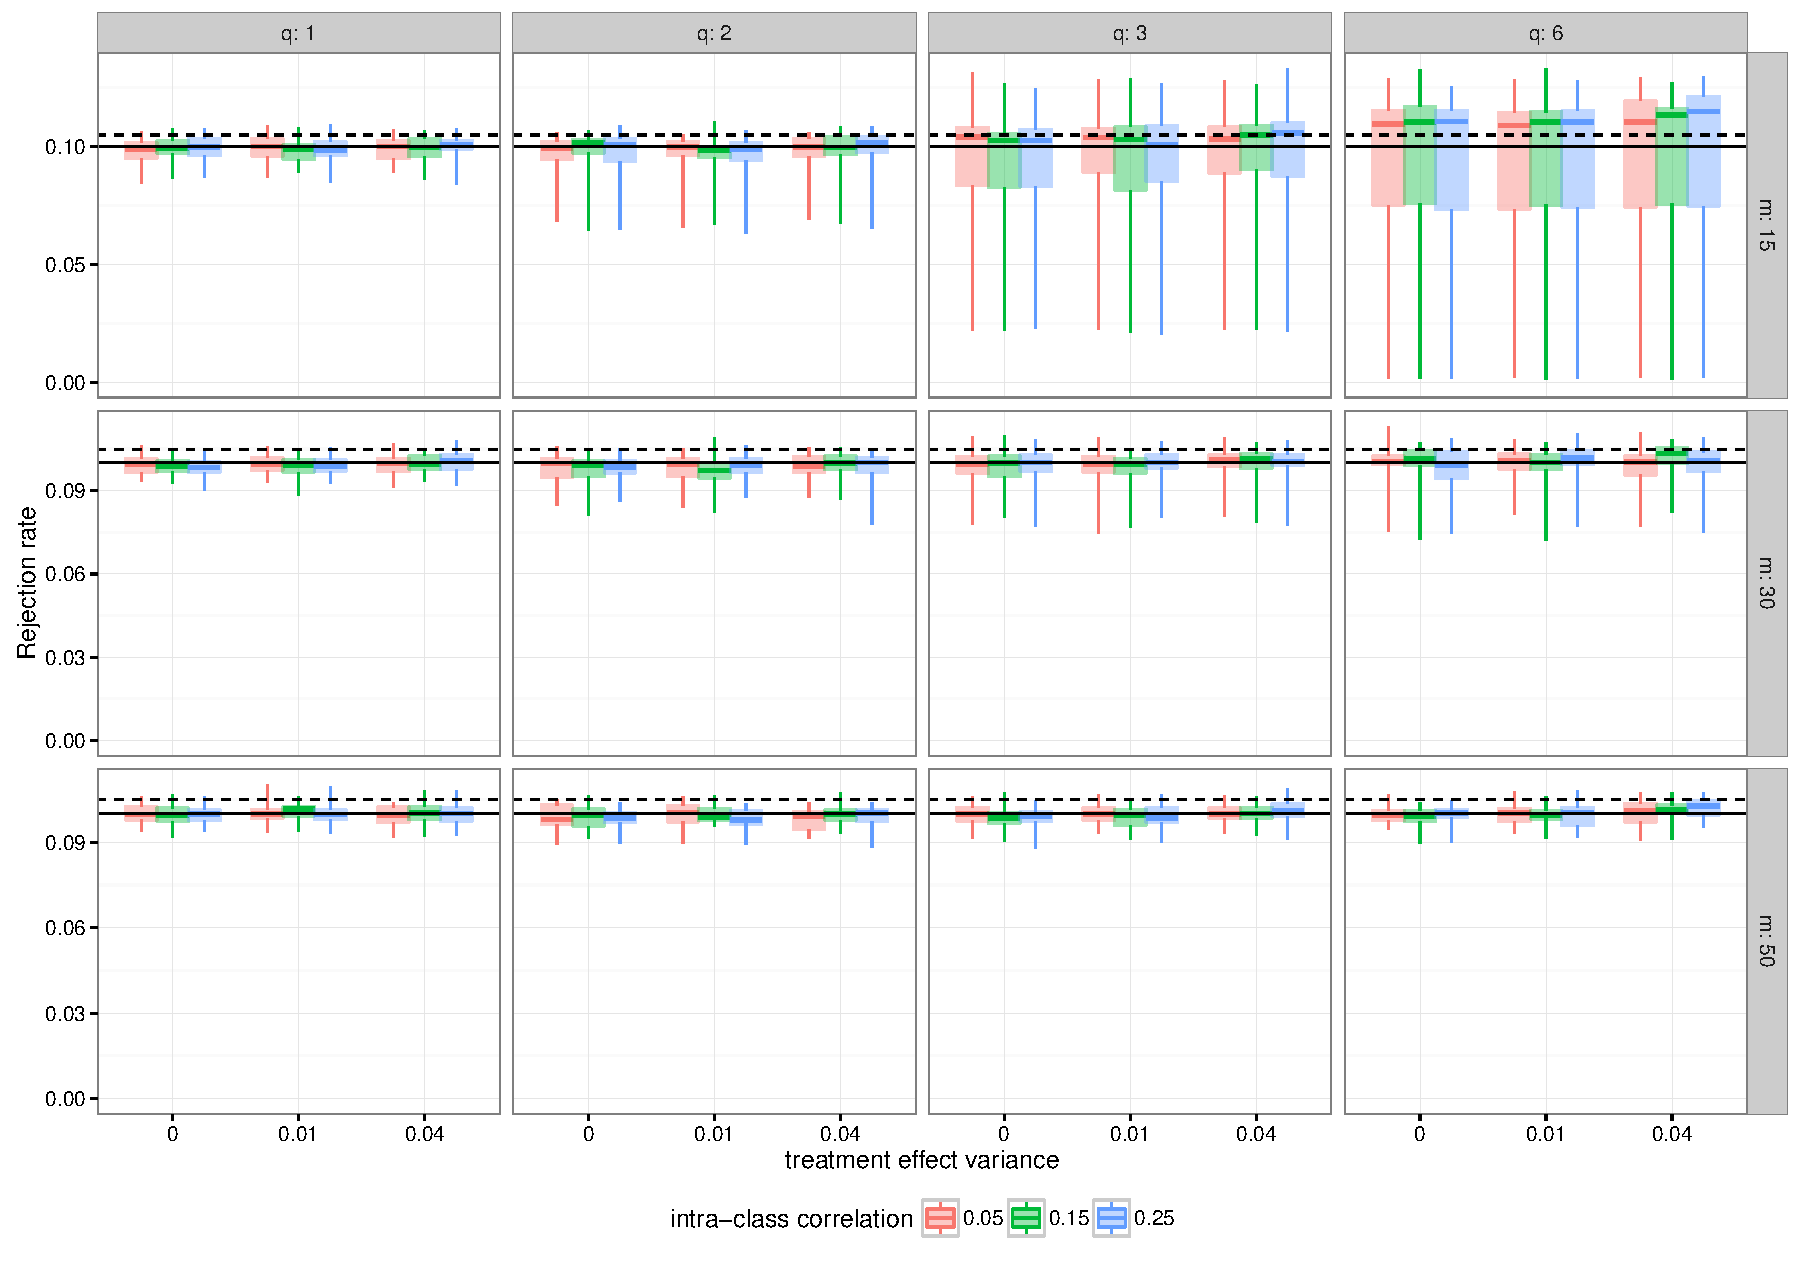
\includegraphics[width=\linewidth]{CR_fig/misspecification_10-1} 

}

\caption[Rejection rates of CR2 AHT test, by treatment effect variance and intra-class correlation for ]{Rejection rates of CR2 AHT test, by treatment effect variance and intra-class correlation for $\alpha = .10$.}\label{fig:misspecification_10}
\end{figure}


\end{knitrout}
\end{landscape}

\bibliographystyle{agsm}
\bibliography{bibliography}

\end{document}
